% Options for packages loaded elsewhere
\PassOptionsToPackage{unicode}{hyperref}
\PassOptionsToPackage{hyphens}{url}
\PassOptionsToPackage{dvipsnames,svgnames,x11names}{xcolor}
%
\documentclass[
  letterpaper,
  DIV=11,
  numbers=noendperiod]{scrreprt}

\usepackage{amsmath,amssymb}
\usepackage{iftex}
\ifPDFTeX
  \usepackage[T1]{fontenc}
  \usepackage[utf8]{inputenc}
  \usepackage{textcomp} % provide euro and other symbols
\else % if luatex or xetex
  \usepackage{unicode-math}
  \defaultfontfeatures{Scale=MatchLowercase}
  \defaultfontfeatures[\rmfamily]{Ligatures=TeX,Scale=1}
\fi
\usepackage{lmodern}
\ifPDFTeX\else  
    % xetex/luatex font selection
\fi
% Use upquote if available, for straight quotes in verbatim environments
\IfFileExists{upquote.sty}{\usepackage{upquote}}{}
\IfFileExists{microtype.sty}{% use microtype if available
  \usepackage[]{microtype}
  \UseMicrotypeSet[protrusion]{basicmath} % disable protrusion for tt fonts
}{}
\usepackage{xcolor}
\setlength{\emergencystretch}{3em} % prevent overfull lines
\setcounter{secnumdepth}{5}
% Make \paragraph and \subparagraph free-standing
\ifx\paragraph\undefined\else
  \let\oldparagraph\paragraph
  \renewcommand{\paragraph}[1]{\oldparagraph{#1}\mbox{}}
\fi
\ifx\subparagraph\undefined\else
  \let\oldsubparagraph\subparagraph
  \renewcommand{\subparagraph}[1]{\oldsubparagraph{#1}\mbox{}}
\fi

\usepackage{color}
\usepackage{fancyvrb}
\newcommand{\VerbBar}{|}
\newcommand{\VERB}{\Verb[commandchars=\\\{\}]}
\DefineVerbatimEnvironment{Highlighting}{Verbatim}{commandchars=\\\{\}}
% Add ',fontsize=\small' for more characters per line
\usepackage{framed}
\definecolor{shadecolor}{RGB}{241,243,245}
\newenvironment{Shaded}{\begin{snugshade}}{\end{snugshade}}
\newcommand{\AlertTok}[1]{\textcolor[rgb]{0.68,0.00,0.00}{#1}}
\newcommand{\AnnotationTok}[1]{\textcolor[rgb]{0.37,0.37,0.37}{#1}}
\newcommand{\AttributeTok}[1]{\textcolor[rgb]{0.40,0.45,0.13}{#1}}
\newcommand{\BaseNTok}[1]{\textcolor[rgb]{0.68,0.00,0.00}{#1}}
\newcommand{\BuiltInTok}[1]{\textcolor[rgb]{0.00,0.23,0.31}{#1}}
\newcommand{\CharTok}[1]{\textcolor[rgb]{0.13,0.47,0.30}{#1}}
\newcommand{\CommentTok}[1]{\textcolor[rgb]{0.37,0.37,0.37}{#1}}
\newcommand{\CommentVarTok}[1]{\textcolor[rgb]{0.37,0.37,0.37}{\textit{#1}}}
\newcommand{\ConstantTok}[1]{\textcolor[rgb]{0.56,0.35,0.01}{#1}}
\newcommand{\ControlFlowTok}[1]{\textcolor[rgb]{0.00,0.23,0.31}{#1}}
\newcommand{\DataTypeTok}[1]{\textcolor[rgb]{0.68,0.00,0.00}{#1}}
\newcommand{\DecValTok}[1]{\textcolor[rgb]{0.68,0.00,0.00}{#1}}
\newcommand{\DocumentationTok}[1]{\textcolor[rgb]{0.37,0.37,0.37}{\textit{#1}}}
\newcommand{\ErrorTok}[1]{\textcolor[rgb]{0.68,0.00,0.00}{#1}}
\newcommand{\ExtensionTok}[1]{\textcolor[rgb]{0.00,0.23,0.31}{#1}}
\newcommand{\FloatTok}[1]{\textcolor[rgb]{0.68,0.00,0.00}{#1}}
\newcommand{\FunctionTok}[1]{\textcolor[rgb]{0.28,0.35,0.67}{#1}}
\newcommand{\ImportTok}[1]{\textcolor[rgb]{0.00,0.46,0.62}{#1}}
\newcommand{\InformationTok}[1]{\textcolor[rgb]{0.37,0.37,0.37}{#1}}
\newcommand{\KeywordTok}[1]{\textcolor[rgb]{0.00,0.23,0.31}{#1}}
\newcommand{\NormalTok}[1]{\textcolor[rgb]{0.00,0.23,0.31}{#1}}
\newcommand{\OperatorTok}[1]{\textcolor[rgb]{0.37,0.37,0.37}{#1}}
\newcommand{\OtherTok}[1]{\textcolor[rgb]{0.00,0.23,0.31}{#1}}
\newcommand{\PreprocessorTok}[1]{\textcolor[rgb]{0.68,0.00,0.00}{#1}}
\newcommand{\RegionMarkerTok}[1]{\textcolor[rgb]{0.00,0.23,0.31}{#1}}
\newcommand{\SpecialCharTok}[1]{\textcolor[rgb]{0.37,0.37,0.37}{#1}}
\newcommand{\SpecialStringTok}[1]{\textcolor[rgb]{0.13,0.47,0.30}{#1}}
\newcommand{\StringTok}[1]{\textcolor[rgb]{0.13,0.47,0.30}{#1}}
\newcommand{\VariableTok}[1]{\textcolor[rgb]{0.07,0.07,0.07}{#1}}
\newcommand{\VerbatimStringTok}[1]{\textcolor[rgb]{0.13,0.47,0.30}{#1}}
\newcommand{\WarningTok}[1]{\textcolor[rgb]{0.37,0.37,0.37}{\textit{#1}}}

\providecommand{\tightlist}{%
  \setlength{\itemsep}{0pt}\setlength{\parskip}{0pt}}\usepackage{longtable,booktabs,array}
\usepackage{calc} % for calculating minipage widths
% Correct order of tables after \paragraph or \subparagraph
\usepackage{etoolbox}
\makeatletter
\patchcmd\longtable{\par}{\if@noskipsec\mbox{}\fi\par}{}{}
\makeatother
% Allow footnotes in longtable head/foot
\IfFileExists{footnotehyper.sty}{\usepackage{footnotehyper}}{\usepackage{footnote}}
\makesavenoteenv{longtable}
\usepackage{graphicx}
\makeatletter
\def\maxwidth{\ifdim\Gin@nat@width>\linewidth\linewidth\else\Gin@nat@width\fi}
\def\maxheight{\ifdim\Gin@nat@height>\textheight\textheight\else\Gin@nat@height\fi}
\makeatother
% Scale images if necessary, so that they will not overflow the page
% margins by default, and it is still possible to overwrite the defaults
% using explicit options in \includegraphics[width, height, ...]{}
\setkeys{Gin}{width=\maxwidth,height=\maxheight,keepaspectratio}
% Set default figure placement to htbp
\makeatletter
\def\fps@figure{htbp}
\makeatother

\KOMAoption{captions}{tableheading}
\makeatletter
\makeatother
\makeatletter
\@ifpackageloaded{bookmark}{}{\usepackage{bookmark}}
\makeatother
\makeatletter
\@ifpackageloaded{caption}{}{\usepackage{caption}}
\AtBeginDocument{%
\ifdefined\contentsname
  \renewcommand*\contentsname{Table of contents}
\else
  \newcommand\contentsname{Table of contents}
\fi
\ifdefined\listfigurename
  \renewcommand*\listfigurename{List of Figures}
\else
  \newcommand\listfigurename{List of Figures}
\fi
\ifdefined\listtablename
  \renewcommand*\listtablename{List of Tables}
\else
  \newcommand\listtablename{List of Tables}
\fi
\ifdefined\figurename
  \renewcommand*\figurename{Figure}
\else
  \newcommand\figurename{Figure}
\fi
\ifdefined\tablename
  \renewcommand*\tablename{Table}
\else
  \newcommand\tablename{Table}
\fi
}
\@ifpackageloaded{float}{}{\usepackage{float}}
\floatstyle{ruled}
\@ifundefined{c@chapter}{\newfloat{codelisting}{h}{lop}}{\newfloat{codelisting}{h}{lop}[chapter]}
\floatname{codelisting}{Listing}
\newcommand*\listoflistings{\listof{codelisting}{List of Listings}}
\makeatother
\makeatletter
\@ifpackageloaded{caption}{}{\usepackage{caption}}
\@ifpackageloaded{subcaption}{}{\usepackage{subcaption}}
\makeatother
\makeatletter
\@ifpackageloaded{tcolorbox}{}{\usepackage[skins,breakable]{tcolorbox}}
\makeatother
\makeatletter
\@ifundefined{shadecolor}{\definecolor{shadecolor}{rgb}{.97, .97, .97}}
\makeatother
\makeatletter
\makeatother
\makeatletter
\makeatother
\ifLuaTeX
  \usepackage{selnolig}  % disable illegal ligatures
\fi
\IfFileExists{bookmark.sty}{\usepackage{bookmark}}{\usepackage{hyperref}}
\IfFileExists{xurl.sty}{\usepackage{xurl}}{} % add URL line breaks if available
\urlstyle{same} % disable monospaced font for URLs
\hypersetup{
  pdftitle={Applying the Histogram of Oriented Gradients Algorithm for Detecting Grass Lay Direction},
  pdfauthor={Ben Sunshine},
  colorlinks=true,
  linkcolor={blue},
  filecolor={Maroon},
  citecolor={Blue},
  urlcolor={Blue},
  pdfcreator={LaTeX via pandoc}}

\title{Applying the Histogram of Oriented Gradients Algorithm for
Detecting Grass Lay Direction}
\author{Ben Sunshine}
\date{2024-01-25}

\begin{document}
\maketitle
\ifdefined\Shaded\renewenvironment{Shaded}{\begin{tcolorbox}[enhanced, boxrule=0pt, breakable, interior hidden, sharp corners, frame hidden, borderline west={3pt}{0pt}{shadecolor}]}{\end{tcolorbox}}\fi

\renewcommand*\contentsname{Table of contents}
{
\hypersetup{linkcolor=}
\setcounter{tocdepth}{2}
\tableofcontents
}
\bookmarksetup{startatroot}

\hypertarget{abstract}{%
\chapter{Abstract}\label{abstract}}

~~~~~~In Alaska, indigenous hunters and gatherers have long observed the
alignment of grass and plants after the growing season as indicative of
prevailing wind directions and shifts. Due to the remote and harsh
conditions, traditional weather stations are absent to measure shifts in
historically predominant wind directions. In a previous study Dr.~Jon
Rosales (Environmental Studies) and his team collected images of grass
lay from St.~Lawrence Island, Alaska, and manually attempted to measure
grass lay angles. This project investigated the Histogram of Oriented
Gradients (HOG) algorithm to automate this process. We applied the
algorithm to various images of grass fields sampled from the internet to
test its viability.

\bookmarksetup{startatroot}

\hypertarget{introduction}{%
\chapter{Introduction}\label{introduction}}

~~~~~~Subsistence-oriented indigenous communities across Alaska rely
heavily on Traditional Ecological Knowledge (TEK), a holistic
understanding of their environment acquired through generations of
observation and cultural transmission. Among the Anishinaabek tradition,
sweetgrass symbolizes wisdom and knowledge, passed down from elders to
younger generations. Indigenous hunters and gatherers have long observed
the alignment of grass and plants after the growing season as indicative
of prevailing wind directions. Predominant wind direction serve a
crucial role to subsistence practitioners when hunting, fishing,
settling, and keeping track of changing weather. On islands like
St.~Lawrence Island in Savoonga, AK, natives have observed a shift from
historically predominant northerly wind patterns to southerly and
easterly and dominated winds. This hypothesis has not yet been
confirmed, due to the absence of weather stations.\\
\hspace*{0.333em}\hspace*{0.333em}\hspace*{0.333em}\hspace*{0.333em}\hspace*{0.333em}\hspace*{0.333em}This
research project seeks to reinforce Traditional Ecological Knowledge
(TEK) with Scientific Ecological Knowledge (SEK) to develop our
understanding of Alaskan indigenous wisdom and its correlation with
modern scientific findings. By employing advanced image processing and
machine learning techniques on imaging data obtained from the Living
Laboratory at St.~Lawrence University, we aim to utilize a Histogram of
Oriented Gradients (HOG) algorithm to enhance the methodology of data
collection and measure the predominant direction in which grass lays
after its growing season. This interdisciplinary approach not only
deepens our comprehension of indigenous knowledge systems but also sheds
light on environmental dynamics and climate change impacts in remote
regions.

\bookmarksetup{startatroot}

\hypertarget{methods}{%
\chapter{Methods}\label{methods}}

~~~~~~The HOG algorithm, introduced by Navneet Dalal and Bill Triggs in
2005, is a popular technique for object detection in images. The
algorithm can identify gradient magnitudes and angles at each pixel in
an image. The preliminary steps involved using the `skimage' library
from Python to preprocess the images of interest. This included loading,
resizing, and converting the images to grayscale. Images were rescaled
to standardize their resolutions and preserve their aspect ratios to
prevent distortion that could affect the accuracy of angle
identification. Converting the images to grayscale was necessary because
it allowed for focusing on a single channel to represent pixel
intensity, rather than three channels (red, green, and blue).\\
\hspace*{0.333em}\hspace*{0.333em}\hspace*{0.333em}\hspace*{0.333em}\hspace*{0.333em}\hspace*{0.333em}The
HOG features were then computed for the resized images, which involved
calculating the gradient magnitudes and angles at each pixel. The
gradient magnitude at each pixel is comprised of the gradients in the
`x' and `y' directions. The gradient in the x-direction is computed by
subtracting the pixel value to the left of pixel of interest is
subtracted from the pixel value to its right. Similarly, the gradient in
the y-direction is calculated by pixel value below the pixel of interest
is subtracted from the pixel value above the pixel of interest. Now to
calculate the gradient magnitude at the pixel of interest, the
Pythagorean Theorem can be utilized where the gradient magnitude is
equal to the square root of the x-gradient squared plus the y-gradient
squared. The angle at a given pixel can be calculated by taking the
inverse tangent of its y-gradient divided by its x-gradient. It is
important to note all angles produced by this algorithm are between zero
and one hundred eighty degrees. This occurs, because the inverse tangent
function used for calculating a given pixel's angle cannot distinguish
between all four quadrants. OR:

\(Magnitude(\mu)=\sqrt{G_{x}^{2} + G_{y}^{2}}\)

\(Angle(\Theta)=\arctan({\frac{G_{y}^{2}}{G_{x}^{2}}})\)

~~~~~~Next, histograms are constructed to visualize the distribution of
gradient magnitudes and angles. Two different techniques for creating
gradient angle histograms were implemented. The simpler method involved
counting the frequencies of angles and The second scheme uses the same
number of bins, but factors in a pixel's gradient magnitude and its
allocation to its bordering bins. Here, the weight assigned to each bin
is calculated by the angle's deviation from the center of its central
bin. This approach allows for a more representative histogram which
splits angles between bins and takes their magnitudes into account.

~~~~~~Lastly, these histograms are converted to polar histograms so the
primary angles can be visualized and compared to their original images.

\bookmarksetup{startatroot}

\hypertarget{results}{%
\chapter{Results}\label{results}}

\hypertarget{load-r-packages}{%
\section{Load R Packages}\label{load-r-packages}}

\begin{Shaded}
\begin{Highlighting}[]
\FunctionTok{library}\NormalTok{(reticulate)}
\FunctionTok{library}\NormalTok{(tidyverse)}
\end{Highlighting}
\end{Shaded}

\begin{verbatim}
-- Attaching core tidyverse packages ------------------------ tidyverse 2.0.0 --
v dplyr     1.1.2     v readr     2.1.4
v forcats   1.0.0     v stringr   1.5.0
v ggplot2   3.5.0     v tibble    3.2.1
v lubridate 1.9.2     v tidyr     1.3.0
v purrr     1.0.2     
-- Conflicts ------------------------------------------ tidyverse_conflicts() --
x dplyr::filter() masks stats::filter()
x dplyr::lag()    masks stats::lag()
i Use the conflicted package (<http://conflicted.r-lib.org/>) to force all conflicts to become errors
\end{verbatim}

\begin{Shaded}
\begin{Highlighting}[]
\FunctionTok{Sys.which}\NormalTok{(}\StringTok{"python"}\NormalTok{)}
\end{Highlighting}
\end{Shaded}

\begin{verbatim}
python 
    "" 
\end{verbatim}

\hypertarget{load-python-libraries}{%
\section{Load Python Libraries}\label{load-python-libraries}}

\begin{Shaded}
\begin{Highlighting}[]

\ImportTok{import}\NormalTok{ matplotlib.pyplot }\ImportTok{as}\NormalTok{ plt}
\ImportTok{import}\NormalTok{ pandas }\ImportTok{as}\NormalTok{ pd}

\CommentTok{\# jupyter only inline output command}
\CommentTok{\#\%matplotlib inline}

\ImportTok{from}\NormalTok{ skimage.io }\ImportTok{import}\NormalTok{ imread, imshow}
\ImportTok{from}\NormalTok{ skimage.transform }\ImportTok{import}\NormalTok{ resize}
\ImportTok{from}\NormalTok{ skimage.feature }\ImportTok{import}\NormalTok{ hog}
\ImportTok{from}\NormalTok{ skimage }\ImportTok{import}\NormalTok{ data, exposure}


\ImportTok{import}\NormalTok{ matplotlib.pyplot }\ImportTok{as}\NormalTok{ plt}
\ImportTok{from}\NormalTok{ skimage }\ImportTok{import}\NormalTok{ io}
\ImportTok{from}\NormalTok{ skimage }\ImportTok{import}\NormalTok{ color}
\ImportTok{from}\NormalTok{ skimage.transform }\ImportTok{import}\NormalTok{ resize}
\ImportTok{import}\NormalTok{ math}
\ImportTok{from}\NormalTok{ skimage.feature }\ImportTok{import}\NormalTok{ hog}
\ImportTok{import}\NormalTok{ numpy }\ImportTok{as}\NormalTok{ np}
\end{Highlighting}
\end{Shaded}

\hypertarget{read-grayscale-resize-image}{%
\section{Read, Grayscale, Resize
Image}\label{read-grayscale-resize-image}}

\begin{Shaded}
\begin{Highlighting}[]
\CommentTok{\# }\AlertTok{TODO}\CommentTok{: DONT CHANGE HEIGHT AND WIDTH}
\NormalTok{img }\OperatorTok{=}\NormalTok{ color.rgb2gray(io.imread(}\StringTok{"images/grass\_image2.jpg"}\NormalTok{))}

\CommentTok{\# img = color.rgb2gray(io.imread("images/b\_test\_image\_copy.jpg"))}
\CommentTok{\#img = color.rgb2gray(io.imread("images/long\_grass\_sample.jpeg"))}
\CommentTok{\#img = color.rgb2gray(io.imread("images/diagnol\_lines.jpg"))}

\CommentTok{\#img = color.rgb2gray(io.imread("images/san\_francisco\_scale\_zoom\_12.png"))}

\CommentTok{\#img = color.rgb2gray(io.imread("images/diagnol\_lines\_flipped.jpg"))}
\CommentTok{\#img = color.rgb2gray(io.imread("images/long\_grass\_sample\_cropped.jpg"))}

\CommentTok{\# aerial rotated image}
\CommentTok{\#img = color.rgb2gray(io.imread("images/living\_lab\_aerial/aerial\_grass\_living\_lab\_rotated.jpg"))}

\CommentTok{\# zoomed internet photo}
\CommentTok{\#img = color.rgb2gray(io.imread("images/dead\_grass\_zoom.jpeg"))}


\CommentTok{\# zoomed in 11}
\CommentTok{\#img = color.rgb2gray(io.imread("images/living\_lab\_aerial/LL\_zoomed\_in\_11.jpg"))}

\CommentTok{\# zoomed in 12}
\CommentTok{\#img = color.rgb2gray(io.imread("images/living\_lab\_aerial/LL\_zoomed\_in\_12.jpg"))}

\CommentTok{\# zoomed in 16}
\CommentTok{\#img = color.rgb2gray(io.imread("images/living\_lab\_aerial/LL\_zoomed\_in\_16\_side.jpg"))}



\CommentTok{\# real one}
\CommentTok{\#img = color.rgb2gray(io.imread("images/living\_labs\_real\_grass\_image.jpg"))}



\NormalTok{img.shape}
\end{Highlighting}
\end{Shaded}

\begin{verbatim}
(395, 596)
\end{verbatim}

\begin{Shaded}
\begin{Highlighting}[]
\CommentTok{\# height = img.shape[0]//5}
\CommentTok{\# width = img.shape[1]//5}

\CommentTok{\# original image aspect ratio}
\NormalTok{aspect\_ratio }\OperatorTok{=}\NormalTok{ img.shape[}\DecValTok{0}\NormalTok{]}\OperatorTok{/}\NormalTok{img.shape[}\DecValTok{1}\NormalTok{]}

\NormalTok{height }\OperatorTok{=} \DecValTok{200}
\NormalTok{width }\OperatorTok{=} \BuiltInTok{int}\NormalTok{(height}\OperatorTok{/}\NormalTok{aspect\_ratio)}
\NormalTok{width }\OperatorTok{=} \DecValTok{300}

\CommentTok{\# height = 128}
\CommentTok{\# width = 192}

\CommentTok{\# make sure the resized is in sample ball park as the original aspect ratio, }
\CommentTok{\# that way the angles don\textquotesingle{}t get squished}
\NormalTok{resized\_ratio }\OperatorTok{=}\NormalTok{ height}\OperatorTok{/}\NormalTok{width}


\NormalTok{img }\OperatorTok{=}\NormalTok{ resize(img, (height, width))}
\CommentTok{\#img = resize(color.rgb2gray(io.imread("b\_test\_image\_copy.jpg")), (height, width))}


\CommentTok{\#resized\_img = resize(img, (height, width))}
\NormalTok{plt.axis(}\StringTok{"off"}\NormalTok{)}
\end{Highlighting}
\end{Shaded}

\begin{verbatim}
(0.0, 1.0, 0.0, 1.0)
\end{verbatim}

\begin{Shaded}
\begin{Highlighting}[]
\NormalTok{plt.imshow(img)}
\BuiltInTok{print}\NormalTok{(img.shape)}
\end{Highlighting}
\end{Shaded}

\begin{verbatim}
(200, 300)
\end{verbatim}

\begin{figure}[H]

{\centering 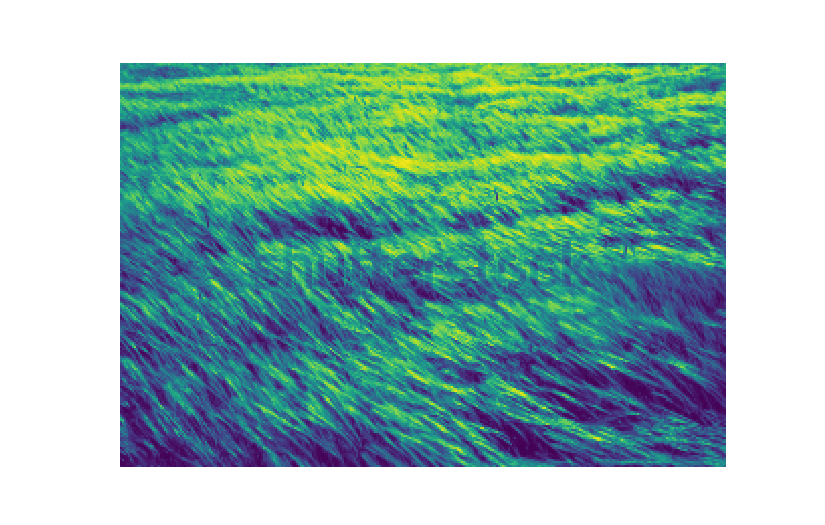
\includegraphics{results_files/figure-pdf/unnamed-chunk-1-1.pdf}

}

\end{figure}

\hypertarget{plot-resized-gray-scale-image}{%
\section{Plot Resized Gray Scale
Image}\label{plot-resized-gray-scale-image}}

\begin{Shaded}
\begin{Highlighting}[]
\NormalTok{plt.figure(figsize}\OperatorTok{=}\NormalTok{(}\DecValTok{15}\NormalTok{, }\DecValTok{8}\NormalTok{))}
\NormalTok{plt.imshow(img, cmap}\OperatorTok{=}\StringTok{"gray"}\NormalTok{)}
\NormalTok{plt.axis(}\StringTok{"off"}\NormalTok{)}
\end{Highlighting}
\end{Shaded}

\begin{verbatim}
(-0.5, 299.5, 199.5, -0.5)
\end{verbatim}

\begin{Shaded}
\begin{Highlighting}[]
\NormalTok{plt.show()}
\end{Highlighting}
\end{Shaded}

\begin{figure}[H]

{\centering 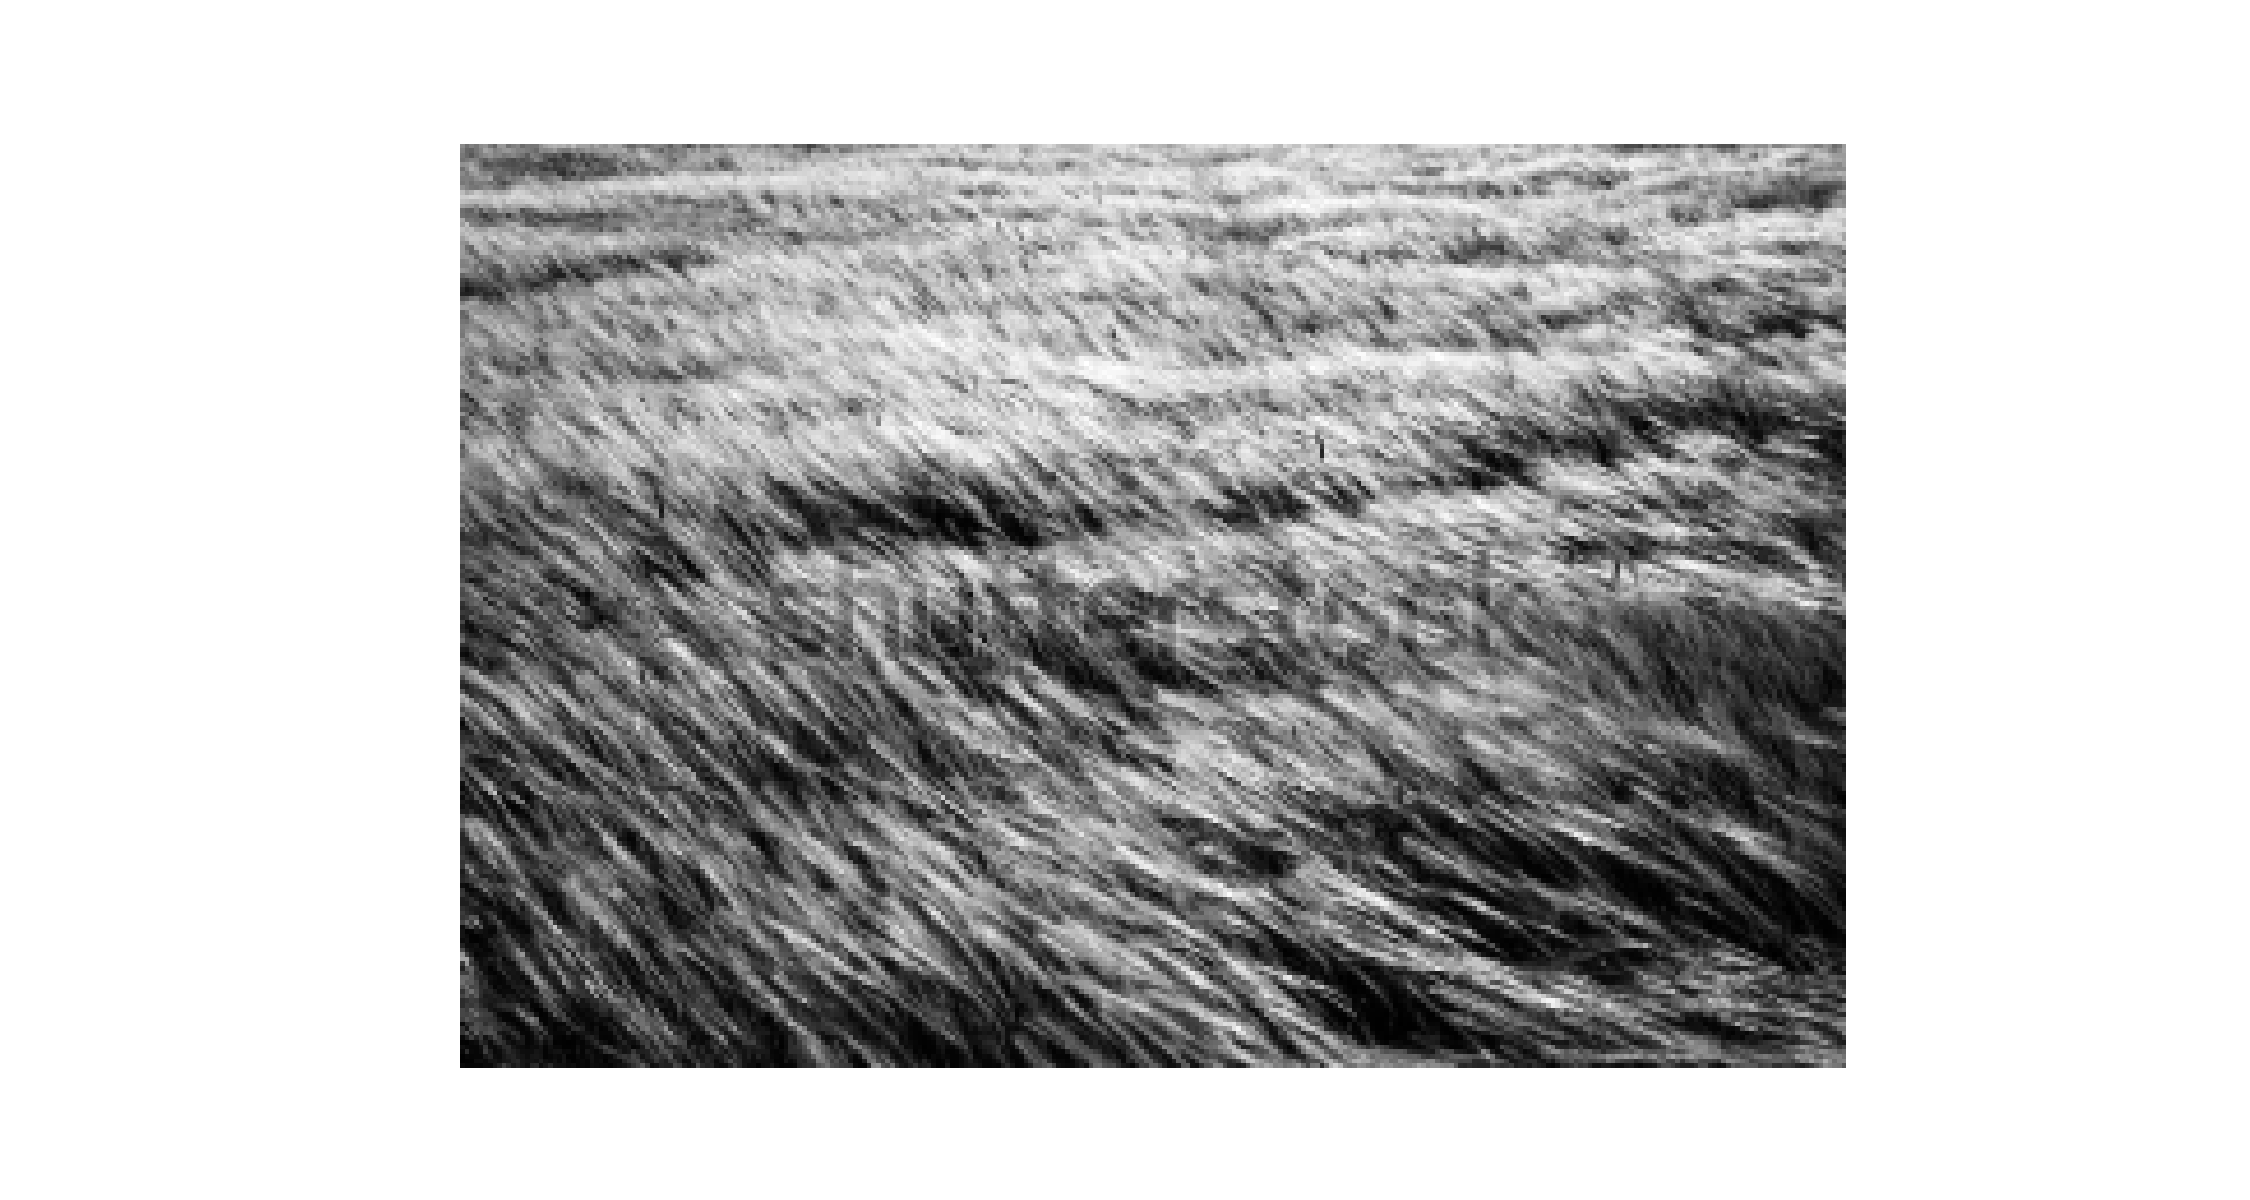
\includegraphics{results_files/figure-pdf/unnamed-chunk-2-3.pdf}

}

\end{figure}

\begin{Shaded}
\begin{Highlighting}[]

\NormalTok{img }\OperatorTok{=}\NormalTok{ np.array(img)}
\end{Highlighting}
\end{Shaded}

\hypertarget{collect-feature-vectors}{%
\section{Collect Feature Vectors}\label{collect-feature-vectors}}

\begin{Shaded}
\begin{Highlighting}[]
\ImportTok{import}\NormalTok{ math}

\NormalTok{mag }\OperatorTok{=}\NormalTok{ []}
\NormalTok{theta }\OperatorTok{=}\NormalTok{ []}

\ControlFlowTok{for}\NormalTok{ i }\KeywordTok{in} \BuiltInTok{range}\NormalTok{(height):}
\NormalTok{    magnitudeArray }\OperatorTok{=}\NormalTok{ []}
\NormalTok{    angleArray }\OperatorTok{=}\NormalTok{ []}
    
    \ControlFlowTok{for}\NormalTok{ j }\KeywordTok{in} \BuiltInTok{range}\NormalTok{(width):}
        \CommentTok{\# Condition for axis 0}
        \ControlFlowTok{if}\NormalTok{ j }\OperatorTok{{-}} \DecValTok{1} \OperatorTok{\textless{}} \DecValTok{0} \KeywordTok{or}\NormalTok{ j }\OperatorTok{+} \DecValTok{1} \OperatorTok{\textgreater{}=}\NormalTok{ width:}
            \ControlFlowTok{if}\NormalTok{ j }\OperatorTok{{-}} \DecValTok{1} \OperatorTok{\textless{}} \DecValTok{0}\NormalTok{:}
                \CommentTok{\# Condition if first element}
\NormalTok{                Gx }\OperatorTok{=}\NormalTok{ img[i][j }\OperatorTok{+} \DecValTok{1}\NormalTok{] }\OperatorTok{{-}} \DecValTok{0}
            \ControlFlowTok{elif}\NormalTok{ j }\OperatorTok{+} \DecValTok{1} \OperatorTok{\textgreater{}=}\NormalTok{ width:}
\NormalTok{                Gx }\OperatorTok{=} \DecValTok{0} \OperatorTok{{-}}\NormalTok{ img[i][j }\OperatorTok{{-}} \DecValTok{1}\NormalTok{]}
        \ControlFlowTok{else}\NormalTok{:}
\NormalTok{            Gx }\OperatorTok{=}\NormalTok{ img[i][j }\OperatorTok{+} \DecValTok{1}\NormalTok{] }\OperatorTok{{-}}\NormalTok{ img[i][j }\OperatorTok{{-}} \DecValTok{1}\NormalTok{]}
        
        \CommentTok{\# Condition for edge case height}
        \ControlFlowTok{if}\NormalTok{ i }\OperatorTok{{-}} \DecValTok{1} \OperatorTok{\textless{}} \DecValTok{0} \KeywordTok{or}\NormalTok{ i }\OperatorTok{+} \DecValTok{1} \OperatorTok{\textgreater{}=}\NormalTok{ height:}
            \ControlFlowTok{if}\NormalTok{ i }\OperatorTok{{-}} \DecValTok{1} \OperatorTok{\textless{}} \DecValTok{0}\NormalTok{:}
\NormalTok{                Gy }\OperatorTok{=} \DecValTok{0} \OperatorTok{{-}}\NormalTok{ img[i }\OperatorTok{+} \DecValTok{1}\NormalTok{][j]}
            \ControlFlowTok{elif}\NormalTok{ i }\OperatorTok{+} \DecValTok{1} \OperatorTok{\textgreater{}=}\NormalTok{ height:}
\NormalTok{                Gy }\OperatorTok{=}\NormalTok{ img[i }\OperatorTok{{-}} \DecValTok{1}\NormalTok{][j] }\OperatorTok{{-}} \DecValTok{0}
        \ControlFlowTok{else}\NormalTok{:}
\NormalTok{            Gy }\OperatorTok{=}\NormalTok{ img[i }\OperatorTok{+} \DecValTok{1}\NormalTok{][j] }\OperatorTok{{-}}\NormalTok{ img[i }\OperatorTok{{-}} \DecValTok{1}\NormalTok{][j]}

        \CommentTok{\# Calculating magnitude}
\NormalTok{        magnitude }\OperatorTok{=}\NormalTok{ math.sqrt(}\BuiltInTok{pow}\NormalTok{(Gx, }\DecValTok{2}\NormalTok{) }\OperatorTok{+} \BuiltInTok{pow}\NormalTok{(Gy, }\DecValTok{2}\NormalTok{))}
\NormalTok{        magnitudeArray.append(}\BuiltInTok{round}\NormalTok{(magnitude, }\DecValTok{9}\NormalTok{))}

        \CommentTok{\# Calculating angle}
        \ControlFlowTok{if}\NormalTok{ Gx }\OperatorTok{==} \DecValTok{0}\NormalTok{:}
\NormalTok{            angle }\OperatorTok{=}\NormalTok{ math.degrees(}\FloatTok{0.0}\NormalTok{)}
        \ControlFlowTok{else}\NormalTok{:}
\NormalTok{            angle }\OperatorTok{=}\NormalTok{ math.degrees(math.atan(Gy }\OperatorTok{/}\NormalTok{ Gx))}
            
            \CommentTok{\# if the angle is negative, need to be between 0 and 360 degrees}
            \ControlFlowTok{if}\NormalTok{ angle }\OperatorTok{\textless{}} \DecValTok{0}\NormalTok{:}
\NormalTok{                angle }\OperatorTok{+=} \DecValTok{180}

\NormalTok{        angleArray.append(}\BuiltInTok{round}\NormalTok{(angle, }\DecValTok{9}\NormalTok{))}
    
\NormalTok{    mag.append(magnitudeArray)}
\NormalTok{    theta.append(angleArray)}
\end{Highlighting}
\end{Shaded}

\begin{Shaded}
\begin{Highlighting}[]
\NormalTok{mag }\OperatorTok{=}\NormalTok{ np.array(mag)}
\NormalTok{theta }\OperatorTok{=}\NormalTok{ np.array(theta)}
\end{Highlighting}
\end{Shaded}

\hypertarget{make-hog-df}{%
\section{Make HOG DF}\label{make-hog-df}}

\begin{Shaded}
\begin{Highlighting}[]
\FunctionTok{hist}\NormalTok{(py}\SpecialCharTok{$}\NormalTok{mag)}
\end{Highlighting}
\end{Shaded}

\begin{figure}[H]

{\centering 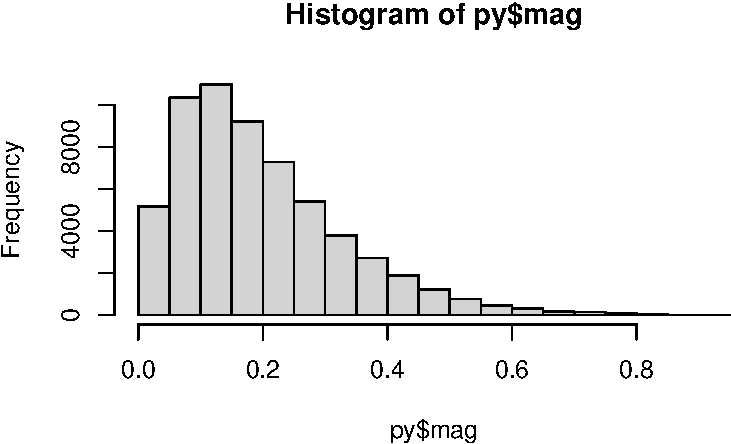
\includegraphics{results_files/figure-pdf/unnamed-chunk-5-5.pdf}

}

\end{figure}

\begin{Shaded}
\begin{Highlighting}[]
\FunctionTok{hist}\NormalTok{(py}\SpecialCharTok{$}\NormalTok{theta)}
\end{Highlighting}
\end{Shaded}

\begin{figure}[H]

{\centering 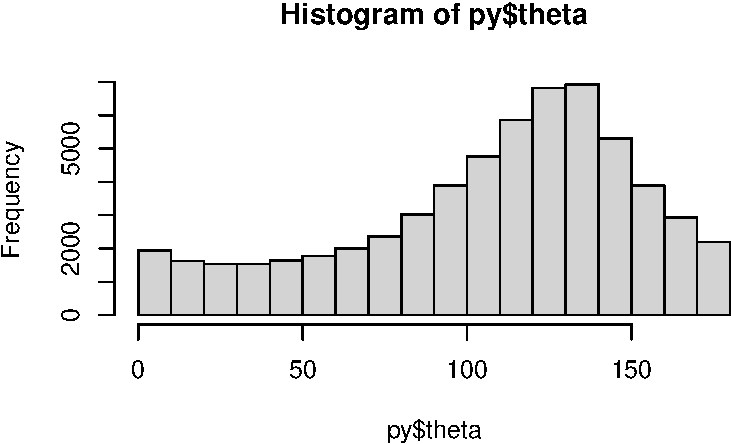
\includegraphics{results_files/figure-pdf/unnamed-chunk-5-6.pdf}

}

\end{figure}

\begin{Shaded}
\begin{Highlighting}[]
\CommentTok{\#as.vector(py$theta)}
\NormalTok{hog\_df }\OtherTok{\textless{}{-}} \FunctionTok{data.frame}\NormalTok{(}\AttributeTok{mag =} \FunctionTok{as.vector}\NormalTok{(py}\SpecialCharTok{$}\NormalTok{mag),}
                     \AttributeTok{theta =} \FunctionTok{as.vector}\NormalTok{((py}\SpecialCharTok{$}\NormalTok{theta))) }\SpecialCharTok{\%\textgreater{}\%}
  \FunctionTok{mutate}\NormalTok{(}\AttributeTok{radian =}\NormalTok{ theta}\SpecialCharTok{*}\NormalTok{(pi}\SpecialCharTok{/}\DecValTok{180}\NormalTok{))}
\end{Highlighting}
\end{Shaded}

\hypertarget{defining-function-for-calculating-hog-neighbors}{%
\section{Defining Function for Calculating HOG
Neighbors}\label{defining-function-for-calculating-hog-neighbors}}

\begin{Shaded}
\begin{Highlighting}[]
\CommentTok{\# Define the number of bins}
\NormalTok{num\_bins }\OtherTok{\textless{}{-}} \DecValTok{9}

\CommentTok{\# Function to calculate the contributions to neighboring bins}
\NormalTok{calculate\_bin\_contributions }\OtherTok{\textless{}{-}} \ControlFlowTok{function}\NormalTok{(angle, magnitude, num\_bins) \{}
\NormalTok{  bin\_width }\OtherTok{\textless{}{-}} \DecValTok{180} \SpecialCharTok{/}\NormalTok{ num\_bins}
\NormalTok{  contributions }\OtherTok{\textless{}{-}} \FunctionTok{numeric}\NormalTok{(num\_bins)}
  
  \CommentTok{\# get the central bin}
\NormalTok{  central\_bin }\OtherTok{\textless{}{-}} \FunctionTok{floor}\NormalTok{(angle }\SpecialCharTok{/}\NormalTok{ bin\_width) }\SpecialCharTok{\%\%}\NormalTok{ num\_bins}
\NormalTok{  next\_bin }\OtherTok{\textless{}{-}}\NormalTok{ (central\_bin }\SpecialCharTok{+} \DecValTok{1}\NormalTok{) }\SpecialCharTok{\%\%}\NormalTok{ num\_bins}
  
  \CommentTok{\# get contributions to neighboring bins}
\NormalTok{  weight }\OtherTok{\textless{}{-}}\NormalTok{ (}\DecValTok{1} \SpecialCharTok{{-}} \FunctionTok{abs}\NormalTok{((angle }\SpecialCharTok{\%\%}\NormalTok{ bin\_width) }\SpecialCharTok{/}\NormalTok{ bin\_width)) }\SpecialCharTok{*}\NormalTok{ magnitude}
  
\NormalTok{  contributions[central\_bin }\SpecialCharTok{+} \DecValTok{1}\NormalTok{] }\OtherTok{\textless{}{-}}\NormalTok{ weight}
\NormalTok{  contributions[next\_bin }\SpecialCharTok{+} \DecValTok{1}\NormalTok{] }\OtherTok{\textless{}{-}}\NormalTok{ magnitude }\SpecialCharTok{{-}}\NormalTok{ weight}
  
  \FunctionTok{return}\NormalTok{(}\FunctionTok{list}\NormalTok{(contributions[}\DecValTok{1}\NormalTok{],}
\NormalTok{         contributions[}\DecValTok{2}\NormalTok{],}
\NormalTok{         contributions[}\DecValTok{3}\NormalTok{],}
\NormalTok{         contributions[}\DecValTok{4}\NormalTok{],}
\NormalTok{         contributions[}\DecValTok{5}\NormalTok{],}
\NormalTok{         contributions[}\DecValTok{6}\NormalTok{],}
\NormalTok{         contributions[}\DecValTok{7}\NormalTok{],}
\NormalTok{         contributions[}\DecValTok{8}\NormalTok{],}
\NormalTok{         contributions[}\DecValTok{9}\NormalTok{])}
\NormalTok{         )}
\NormalTok{\}}


\CommentTok{\# test}
\NormalTok{angle }\OtherTok{\textless{}{-}} \DecValTok{170}
\NormalTok{magnitude }\OtherTok{\textless{}{-}} \DecValTok{1}
\NormalTok{bin\_contributions }\OtherTok{\textless{}{-}} \FunctionTok{calculate\_bin\_contributions}\NormalTok{(angle, magnitude, num\_bins)}
\NormalTok{bin\_contributions}
\end{Highlighting}
\end{Shaded}

\begin{verbatim}
[[1]]
[1] 0.5

[[2]]
[1] 0

[[3]]
[1] 0

[[4]]
[1] 0

[[5]]
[1] 0

[[6]]
[1] 0

[[7]]
[1] 0

[[8]]
[1] 0

[[9]]
[1] 0.5
\end{verbatim}

\begin{Shaded}
\begin{Highlighting}[]
\NormalTok{bin\_contributions[}\DecValTok{9}\NormalTok{]}
\end{Highlighting}
\end{Shaded}

\begin{verbatim}
[[1]]
[1] 0.5
\end{verbatim}

\begin{Shaded}
\begin{Highlighting}[]
\NormalTok{bin\_contributions[}\DecValTok{1}\NormalTok{]}
\end{Highlighting}
\end{Shaded}

\begin{verbatim}
[[1]]
[1] 0.5
\end{verbatim}

\begin{Shaded}
\begin{Highlighting}[]
\NormalTok{contribution\_hog\_df }\OtherTok{\textless{}{-}} \FunctionTok{data.frame}\NormalTok{(}\AttributeTok{mag =} \FunctionTok{as.vector}\NormalTok{(py}\SpecialCharTok{$}\NormalTok{mag),}
                     \AttributeTok{theta =} \FunctionTok{as.vector}\NormalTok{((py}\SpecialCharTok{$}\NormalTok{theta))) }\SpecialCharTok{\%\textgreater{}\%}
  \FunctionTok{mutate}\NormalTok{(}\AttributeTok{radian =}\NormalTok{ theta}\SpecialCharTok{*}\NormalTok{(pi}\SpecialCharTok{/}\DecValTok{180}\NormalTok{)) }\SpecialCharTok{\%\textgreater{}\%}
  \FunctionTok{filter}\NormalTok{(mag }\SpecialCharTok{\textgreater{}} \FloatTok{0.1}\NormalTok{) }\SpecialCharTok{\%\textgreater{}\%}
  \FunctionTok{rowwise}\NormalTok{() }\SpecialCharTok{\%\textgreater{}\%}
  \FunctionTok{mutate}\NormalTok{(}\StringTok{\textasciigrave{}}\AttributeTok{0}\StringTok{\textasciigrave{}} \OtherTok{=} \FunctionTok{calculate\_bin\_contributions}\NormalTok{(theta, mag, }\DecValTok{9}\NormalTok{)[[}\DecValTok{1}\NormalTok{]],}
         \StringTok{\textasciigrave{}}\AttributeTok{20}\StringTok{\textasciigrave{}} \OtherTok{=} \FunctionTok{calculate\_bin\_contributions}\NormalTok{(theta, mag, }\DecValTok{9}\NormalTok{)[[}\DecValTok{2}\NormalTok{]],}
         \StringTok{\textasciigrave{}}\AttributeTok{40}\StringTok{\textasciigrave{}} \OtherTok{=} \FunctionTok{calculate\_bin\_contributions}\NormalTok{(theta, mag, }\DecValTok{9}\NormalTok{)[[}\DecValTok{3}\NormalTok{]],}
         \StringTok{\textasciigrave{}}\AttributeTok{60}\StringTok{\textasciigrave{}} \OtherTok{=} \FunctionTok{calculate\_bin\_contributions}\NormalTok{(theta, mag, }\DecValTok{9}\NormalTok{)[[}\DecValTok{4}\NormalTok{]],}
         \StringTok{\textasciigrave{}}\AttributeTok{80}\StringTok{\textasciigrave{}} \OtherTok{=} \FunctionTok{calculate\_bin\_contributions}\NormalTok{(theta, mag, }\DecValTok{9}\NormalTok{)[[}\DecValTok{5}\NormalTok{]],}
         \StringTok{\textasciigrave{}}\AttributeTok{100}\StringTok{\textasciigrave{}} \OtherTok{=} \FunctionTok{calculate\_bin\_contributions}\NormalTok{(theta, mag, }\DecValTok{9}\NormalTok{)[[}\DecValTok{6}\NormalTok{]],}
         \StringTok{\textasciigrave{}}\AttributeTok{120}\StringTok{\textasciigrave{}} \OtherTok{=} \FunctionTok{calculate\_bin\_contributions}\NormalTok{(theta, mag, }\DecValTok{9}\NormalTok{)[[}\DecValTok{7}\NormalTok{]],}
         \StringTok{\textasciigrave{}}\AttributeTok{140}\StringTok{\textasciigrave{}} \OtherTok{=} \FunctionTok{calculate\_bin\_contributions}\NormalTok{(theta, mag, }\DecValTok{9}\NormalTok{)[[}\DecValTok{8}\NormalTok{]],}
         \StringTok{\textasciigrave{}}\AttributeTok{160}\StringTok{\textasciigrave{}} \OtherTok{=} \FunctionTok{calculate\_bin\_contributions}\NormalTok{(theta, mag, }\DecValTok{9}\NormalTok{)[[}\DecValTok{9}\NormalTok{]],}
\NormalTok{         )}

\CommentTok{\# split\_histo\_df \textless{}{-} hog\_df[4:ncol(hog\_df)] \%\textgreater{}\%}
\NormalTok{split\_histo\_df }\OtherTok{\textless{}{-}}\NormalTok{ contribution\_hog\_df }\SpecialCharTok{\%\textgreater{}\%}
  \FunctionTok{pivot\_longer}\NormalTok{(}\AttributeTok{names\_to =} \StringTok{"bin"}\NormalTok{, }\AttributeTok{values\_to =} \StringTok{"contribution"}\NormalTok{, }\AttributeTok{cols =} \DecValTok{4}\SpecialCharTok{:}\FunctionTok{ncol}\NormalTok{(hog\_df)) }\SpecialCharTok{\%\textgreater{}\%}
  \FunctionTok{mutate}\NormalTok{(}\AttributeTok{bin =} \FunctionTok{as.numeric}\NormalTok{(bin))}
\end{Highlighting}
\end{Shaded}

\begin{verbatim}
Warning: There was 1 warning in `mutate()`.
i In argument: `bin = as.numeric(bin)`.
Caused by warning:
! NAs introduced by coercion
\end{verbatim}

\begin{Shaded}
\begin{Highlighting}[]
\NormalTok{split\_histo\_df }\OtherTok{\textless{}{-}}
\NormalTok{  split\_histo\_df }\SpecialCharTok{\%\textgreater{}\%}
  \FunctionTok{group\_by}\NormalTok{(bin) }\SpecialCharTok{\%\textgreater{}\%}
  \FunctionTok{summarise}\NormalTok{(}\AttributeTok{contribution\_sum =} \FunctionTok{sum}\NormalTok{(contribution))}



\NormalTok{polar\_split\_plot }\OtherTok{\textless{}{-}}
  \FunctionTok{ggplot}\NormalTok{(split\_histo\_df, }\CommentTok{\#\textgreater{}\% filter(mag \textgreater{}= 0.3), }
         \FunctionTok{aes}\NormalTok{(}\AttributeTok{x =}\NormalTok{ bin, }\AttributeTok{y =}\NormalTok{ contribution\_sum)) }\SpecialCharTok{+}
  \CommentTok{\# geom\_histogram(stat = "identity", }
  \CommentTok{\#                colour = "black", }
  \CommentTok{\#                fill = "lightblue", }
  \CommentTok{\#                breaks = seq(0, 360, length.out = 30),}
  \CommentTok{\#                bins = 9) +}
  \FunctionTok{geom\_histogram}\NormalTok{(}\AttributeTok{stat =} \StringTok{"identity"}\NormalTok{,}
                 \AttributeTok{colour =} \StringTok{"black"}\NormalTok{, }
                 \AttributeTok{fill =} \StringTok{"lightblue"}\NormalTok{, }
                 \AttributeTok{breaks =} \FunctionTok{seq}\NormalTok{(}\DecValTok{0}\NormalTok{, }\DecValTok{360}\NormalTok{, }\AttributeTok{length.out =} \FloatTok{17.5}\NormalTok{),}
                 \AttributeTok{bins =} \DecValTok{9}\NormalTok{) }\SpecialCharTok{+}
  \FunctionTok{coord\_polar}\NormalTok{(}
    \AttributeTok{theta =} \StringTok{"x"}\NormalTok{, }\AttributeTok{start =} \DecValTok{0}\NormalTok{, }\AttributeTok{direction =} \DecValTok{1}\NormalTok{) }\SpecialCharTok{+}
  \FunctionTok{scale\_x\_continuous}\NormalTok{(}\AttributeTok{limits =} \FunctionTok{c}\NormalTok{(}\DecValTok{0}\NormalTok{,}\DecValTok{360}\NormalTok{),}
    \AttributeTok{breaks =} \FunctionTok{c}\NormalTok{(}\DecValTok{0}\NormalTok{, }\DecValTok{45}\NormalTok{, }\DecValTok{90}\NormalTok{, }\DecValTok{135}\NormalTok{, }\DecValTok{180}\NormalTok{, }\DecValTok{225}\NormalTok{, }\DecValTok{270}\NormalTok{, }\DecValTok{315}\NormalTok{), }
    \AttributeTok{labels =} \FunctionTok{c}\NormalTok{(}\StringTok{"N"}\NormalTok{, }\StringTok{"NE"}\NormalTok{, }\StringTok{"E"}\NormalTok{, }\StringTok{"SE"}\NormalTok{, }\StringTok{"S"}\NormalTok{, }\StringTok{"SW"}\NormalTok{, }\StringTok{"W"}\NormalTok{, }\StringTok{"NW"}\NormalTok{)}
\NormalTok{  )}\SpecialCharTok{+}
  \FunctionTok{labs}\NormalTok{(}\AttributeTok{title =} \StringTok{"Polar Plot of Internet Grass Image}\SpecialCharTok{\textbackslash{}n}\StringTok{Using Distributed HOG Technique"}\NormalTok{) }\SpecialCharTok{+}
  \FunctionTok{theme\_minimal}\NormalTok{() }\SpecialCharTok{+}
  \FunctionTok{labs}\NormalTok{(}\AttributeTok{x =} \StringTok{""}\NormalTok{) }\SpecialCharTok{+}
  \FunctionTok{theme}\NormalTok{(}\AttributeTok{axis.title.y =} \FunctionTok{element\_blank}\NormalTok{(),}
        \AttributeTok{plot.title =} \FunctionTok{element\_text}\NormalTok{(}\AttributeTok{hjust =} \FloatTok{0.5}\NormalTok{))}
\end{Highlighting}
\end{Shaded}

\begin{verbatim}
Warning in geom_histogram(stat = "identity", colour = "black", fill =
"lightblue", : Ignoring unknown parameters: `binwidth`, `bins`, `pad`, and
`breaks`
\end{verbatim}

\begin{Shaded}
\begin{Highlighting}[]
\NormalTok{polar\_split\_plot}
\end{Highlighting}
\end{Shaded}

\begin{verbatim}
Warning: Removed 2 rows containing missing values or values outside the scale range
(`geom_bar()`).
\end{verbatim}

\begin{figure}[H]

{\centering 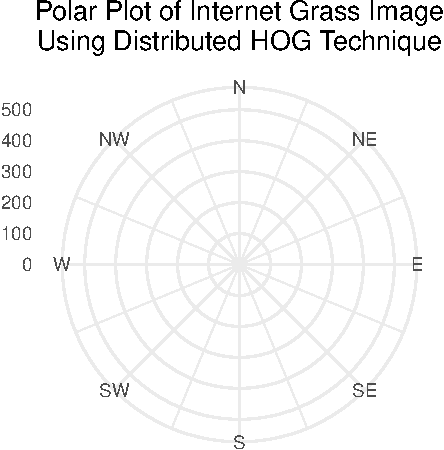
\includegraphics{results_files/figure-pdf/unnamed-chunk-6-1.pdf}

}

\end{figure}

\hypertarget{create-histogram-plots-of-gradient-magnitudes-and-angles}{%
\section{Create Histogram Plots of Gradient Magnitudes and
Angles}\label{create-histogram-plots-of-gradient-magnitudes-and-angles}}

\begin{Shaded}
\begin{Highlighting}[]
\NormalTok{histogram\_mag\_plot }\OtherTok{\textless{}{-}}
  \FunctionTok{ggplot}\NormalTok{(hog\_df, }\FunctionTok{aes}\NormalTok{(}\AttributeTok{x =}\NormalTok{ mag)) }\SpecialCharTok{+}
  \FunctionTok{geom\_histogram}\NormalTok{(}\AttributeTok{colour =} \StringTok{"black"}\NormalTok{, }\AttributeTok{fill =} \StringTok{"lightblue"}\NormalTok{) }\SpecialCharTok{+}
  \FunctionTok{scale\_x\_continuous}\NormalTok{() }\SpecialCharTok{+} 
  \FunctionTok{labs}\NormalTok{(}\AttributeTok{x =} \StringTok{"Gradient Magnitude"}\NormalTok{, }\AttributeTok{y =} \StringTok{"Count"}\CommentTok{\#, title = "Histogram of Magnitudes of Gradients"}
\NormalTok{       ) }\SpecialCharTok{+}
  \FunctionTok{theme\_minimal}\NormalTok{() }\SpecialCharTok{+}
  \FunctionTok{theme}\NormalTok{(}\AttributeTok{plot.title =} \FunctionTok{element\_text}\NormalTok{(}\AttributeTok{hjust =} \FloatTok{0.5}\NormalTok{))}

\NormalTok{histogram\_mag\_plot}
\end{Highlighting}
\end{Shaded}

\begin{verbatim}
`stat_bin()` using `bins = 30`. Pick better value with `binwidth`.
\end{verbatim}

\begin{figure}[H]

{\centering 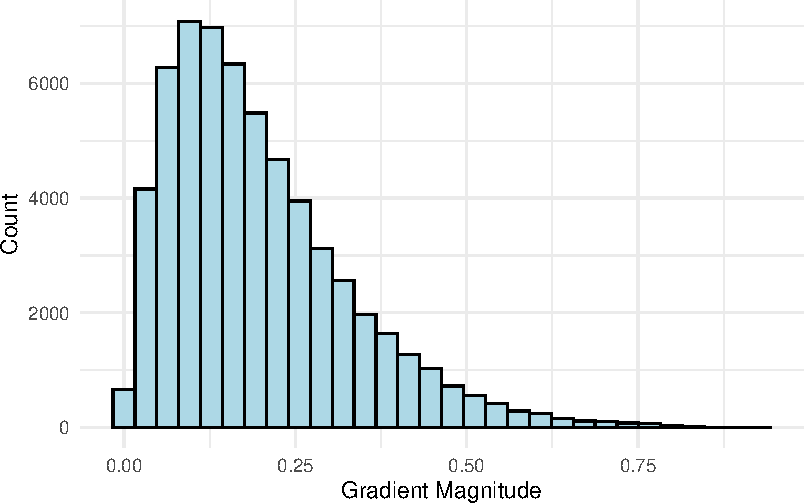
\includegraphics{results_files/figure-pdf/unnamed-chunk-7-1.pdf}

}

\end{figure}

\begin{Shaded}
\begin{Highlighting}[]
\FunctionTok{ggsave}\NormalTok{(}\StringTok{"images/plots/grass2\_magnitude\_histogram.jpg"}\NormalTok{, histogram\_mag\_plot, }\AttributeTok{width =} \DecValTok{6}\NormalTok{, }\AttributeTok{height =} \DecValTok{4}\NormalTok{, }\AttributeTok{dpi =} \DecValTok{300}\NormalTok{)}
\end{Highlighting}
\end{Shaded}

\begin{verbatim}
`stat_bin()` using `bins = 30`. Pick better value with `binwidth`.
\end{verbatim}

\begin{Shaded}
\begin{Highlighting}[]
\NormalTok{histogram\_theta\_plot }\OtherTok{\textless{}{-}}
  \FunctionTok{ggplot}\NormalTok{(hog\_df, }\FunctionTok{aes}\NormalTok{(}\AttributeTok{x =}\NormalTok{ theta)) }\SpecialCharTok{+}
  \FunctionTok{geom\_histogram}\NormalTok{(}\AttributeTok{binwidth =} \DecValTok{10}\NormalTok{, }\AttributeTok{colour =} \StringTok{"black"}\NormalTok{, }\AttributeTok{fill =} \StringTok{"lightblue"}\NormalTok{) }\SpecialCharTok{+}
  \FunctionTok{scale\_x\_continuous}\NormalTok{(}\AttributeTok{breaks =} \FunctionTok{c}\NormalTok{(}\DecValTok{0}\NormalTok{,}\DecValTok{20}\NormalTok{,}\DecValTok{40}\NormalTok{,}\DecValTok{60}\NormalTok{,}\DecValTok{80}\NormalTok{,}\DecValTok{100}\NormalTok{,}\DecValTok{120}\NormalTok{,}\DecValTok{140}\NormalTok{,}\DecValTok{160}\NormalTok{,}\DecValTok{180}\NormalTok{)) }\SpecialCharTok{+} 
  \FunctionTok{labs}\NormalTok{(}\AttributeTok{x =} \StringTok{"Angle (Degrees)"}\NormalTok{, }\AttributeTok{y =} \StringTok{"Count"}\CommentTok{\#, title = "Simple Histogram of Oriented Gradients"}
\NormalTok{       ) }\SpecialCharTok{+}
  \FunctionTok{theme\_minimal}\NormalTok{() }\SpecialCharTok{+}
  \FunctionTok{theme}\NormalTok{(}\AttributeTok{plot.title =} \FunctionTok{element\_text}\NormalTok{(}\AttributeTok{hjust =} \FloatTok{0.5}\NormalTok{))}

\NormalTok{histogram\_theta\_plot}
\end{Highlighting}
\end{Shaded}

\begin{figure}[H]

{\centering 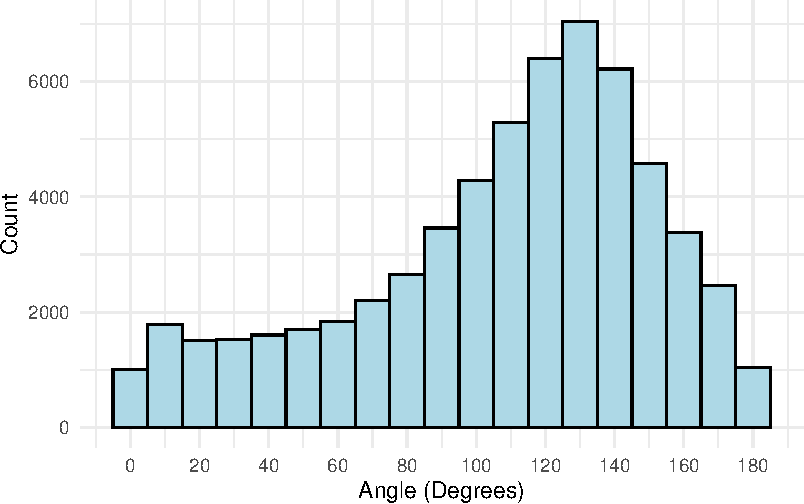
\includegraphics{results_files/figure-pdf/unnamed-chunk-7-2.pdf}

}

\end{figure}

\begin{Shaded}
\begin{Highlighting}[]
\FunctionTok{ggsave}\NormalTok{(}\StringTok{"images/plots/grass2\_angles\_histogram.jpg"}\NormalTok{, histogram\_theta\_plot, }\AttributeTok{width =} \DecValTok{6}\NormalTok{, }\AttributeTok{height =} \DecValTok{4}\NormalTok{, }\AttributeTok{dpi =} \DecValTok{300}\NormalTok{)}
\end{Highlighting}
\end{Shaded}

\hypertarget{plot-magnitudes-as-image}{%
\section{Plot Magnitudes as Image}\label{plot-magnitudes-as-image}}

\begin{Shaded}
\begin{Highlighting}[]
\ImportTok{import}\NormalTok{ matplotlib.pyplot }\ImportTok{as}\NormalTok{ plt}

\NormalTok{plt.figure(figsize}\OperatorTok{=}\NormalTok{(}\DecValTok{15}\NormalTok{, }\DecValTok{8}\NormalTok{))}
\CommentTok{\# plt.title(\textquotesingle{}Gradient Magnitudes by Pixel\textquotesingle{})  \# Corrected line}
\CommentTok{\# plt.suptitle("Image 3", y=0.75, fontsize=18)}
\NormalTok{plt.imshow(mag, cmap}\OperatorTok{=}\StringTok{"gray"}\NormalTok{)}
\NormalTok{plt.axis(}\StringTok{"off"}\NormalTok{)}
\end{Highlighting}
\end{Shaded}

\begin{verbatim}
(-0.5, 299.5, 199.5, -0.5)
\end{verbatim}

\begin{Shaded}
\begin{Highlighting}[]
\NormalTok{plt.show()}
\end{Highlighting}
\end{Shaded}

\begin{figure}[H]

{\centering 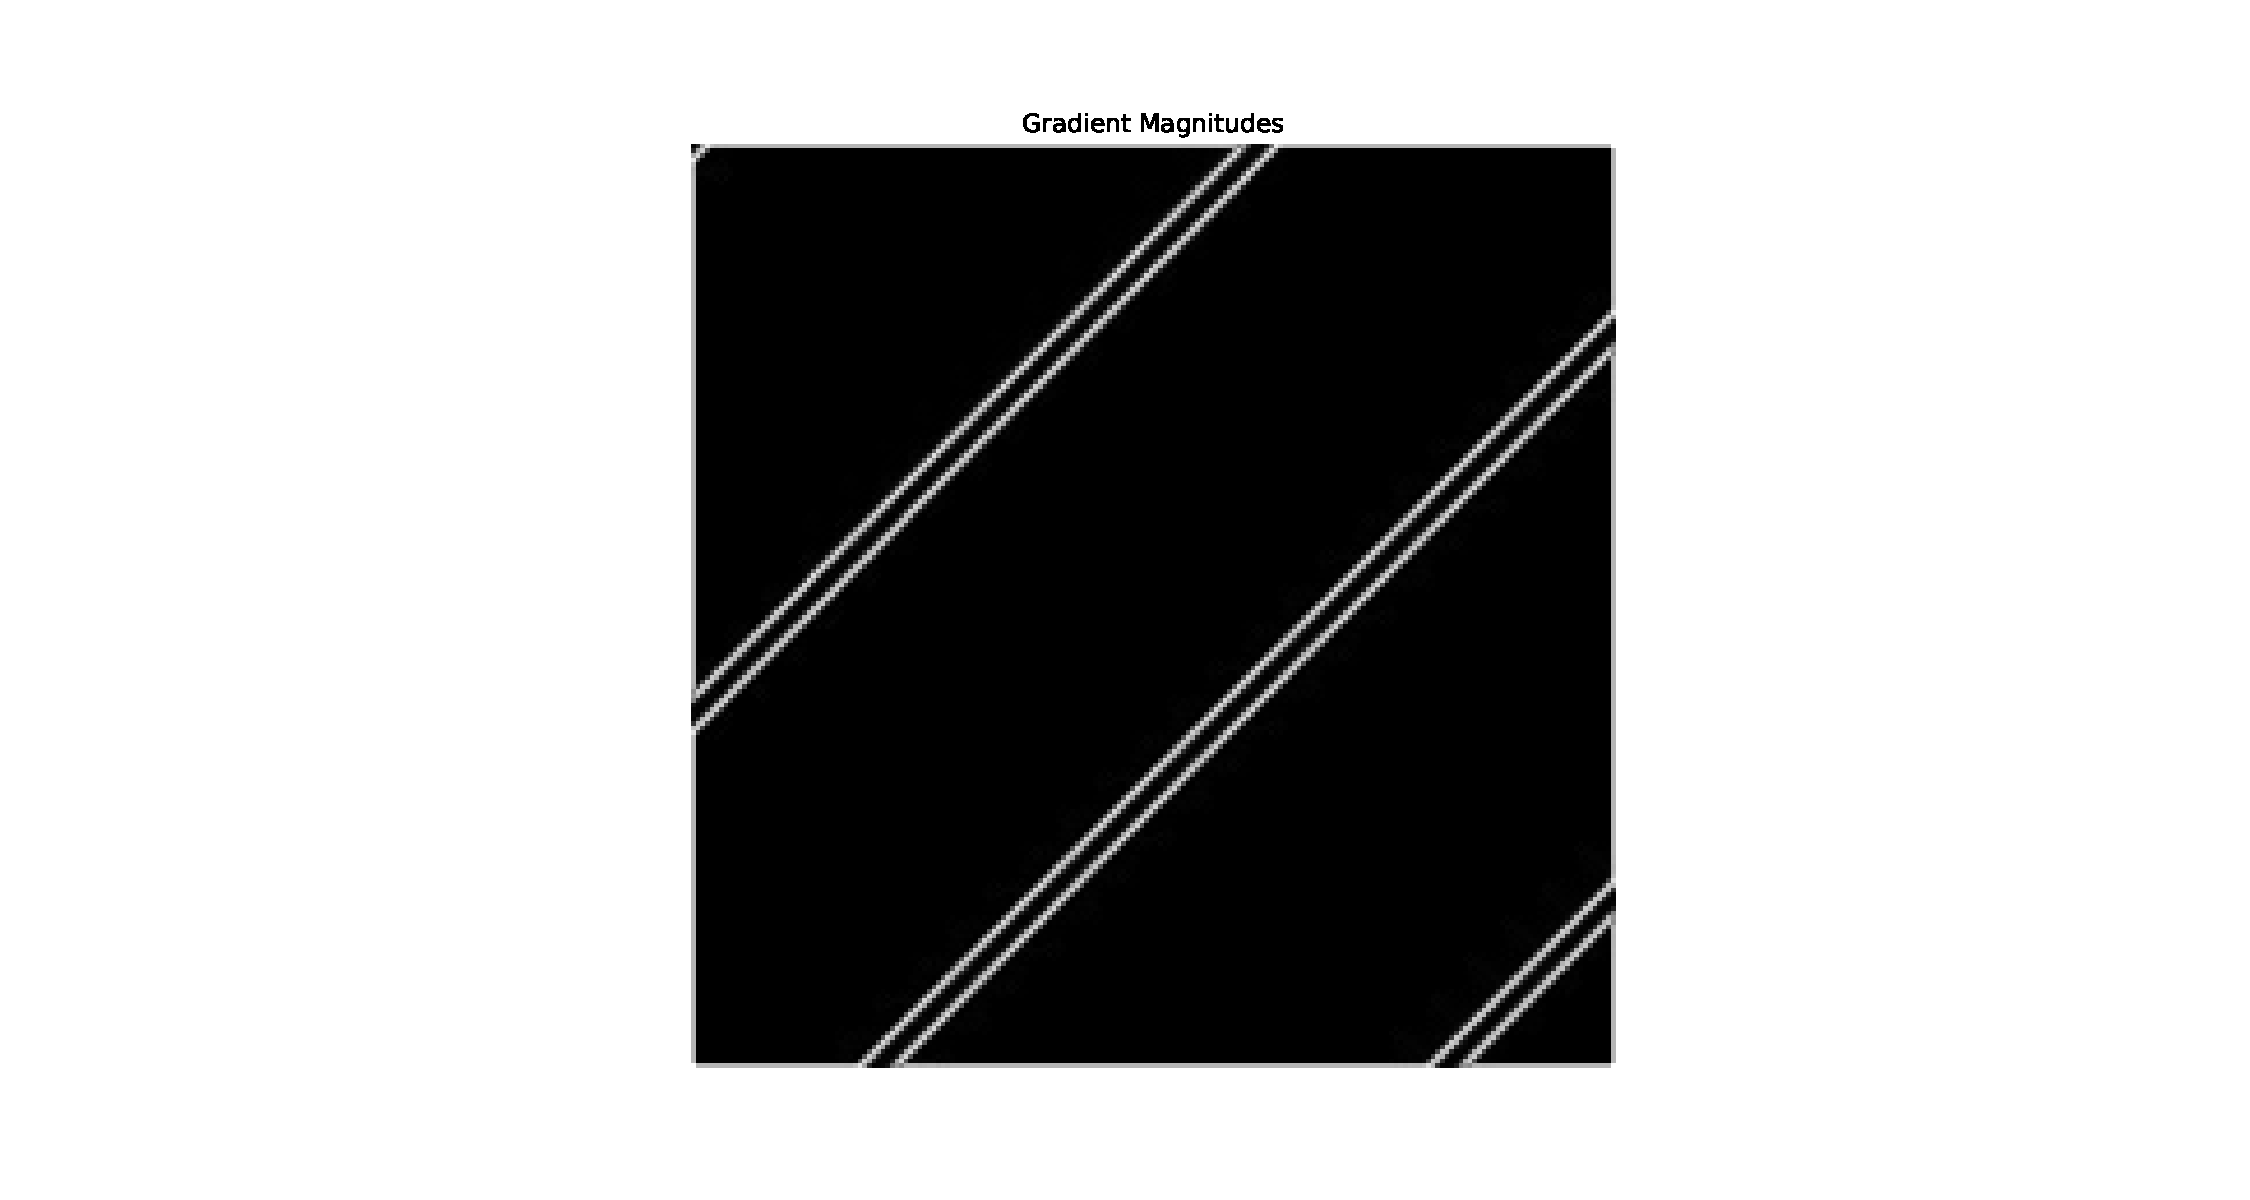
\includegraphics{results_files/figure-pdf/unnamed-chunk-8-1.pdf}

}

\end{figure}

\begin{Shaded}
\begin{Highlighting}[]

\NormalTok{plt.savefig(}\StringTok{"mag.png"}\NormalTok{, dpi}\OperatorTok{=}\DecValTok{300}\NormalTok{)}
\end{Highlighting}
\end{Shaded}

\begin{figure}[H]

{\centering 
\includegraphics{results_files/figure-pdf/unnamed-chunk-8-2.pdf}

}

\end{figure}

\begin{Shaded}
\begin{Highlighting}[]
\NormalTok{number\_of\_bins }\OperatorTok{=} \DecValTok{9}
\NormalTok{step\_size }\OperatorTok{=} \DecValTok{180} \OperatorTok{/}\NormalTok{ number\_of\_bins}
\end{Highlighting}
\end{Shaded}

\begin{Shaded}
\begin{Highlighting}[]
\CommentTok{\#Function to calculate the value of centre of jth bin}
\KeywordTok{def}\NormalTok{ calculate\_j(angle):}
\NormalTok{  temp }\OperatorTok{=}\NormalTok{ (angle }\OperatorTok{/}\NormalTok{ step\_size) }\OperatorTok{{-}} \FloatTok{0.5}
\NormalTok{  j }\OperatorTok{=}\NormalTok{ math.floor(temp)}
  \ControlFlowTok{return}\NormalTok{ j}
\end{Highlighting}
\end{Shaded}

\begin{Shaded}
\begin{Highlighting}[]
\CommentTok{\# Function to calculate the value of jth bin}
\KeywordTok{def}\NormalTok{ calculate\_Cj(j):}
\NormalTok{  Cj }\OperatorTok{=}\NormalTok{ step\_size }\OperatorTok{*}\NormalTok{ (j }\OperatorTok{+} \FloatTok{0.5}\NormalTok{)}
  \ControlFlowTok{return} \BuiltInTok{round}\NormalTok{(Cj, }\DecValTok{9}\NormalTok{)}
\end{Highlighting}
\end{Shaded}

\begin{Shaded}
\begin{Highlighting}[]
\CommentTok{\# }
\KeywordTok{def}\NormalTok{ calculate\_value\_j(magnitude, angle, j):}
\NormalTok{  Cj }\OperatorTok{=}\NormalTok{ calculate\_Cj(j}\OperatorTok{+}\DecValTok{1}\NormalTok{)}
\NormalTok{  Vj }\OperatorTok{=}\NormalTok{ magnitude }\OperatorTok{*}\NormalTok{ ((Cj }\OperatorTok{{-}}\NormalTok{ angle) }\OperatorTok{/}\NormalTok{ step\_size)}
  \ControlFlowTok{return} \BuiltInTok{round}\NormalTok{(Vj, }\DecValTok{9}\NormalTok{)}
\end{Highlighting}
\end{Shaded}

\begin{Shaded}
\begin{Highlighting}[]
\NormalTok{histogram\_points\_nine }\OperatorTok{=}\NormalTok{ []}
\NormalTok{high\_val }\OperatorTok{=} \DecValTok{10}
\CommentTok{\# for i in range(0, height, high\_val):}
\CommentTok{\#   temp = []}
\CommentTok{\#   for j in range(0, width, high\_val):}
\CommentTok{\#     magnitude\_values = [[mag[i][x] for x in range(j, j+high\_val)] for i in range(i,i+high\_val)]}
\CommentTok{\#     angle\_values = [[theta[i][x] for x in range(j, j+high\_val)] for i in range(i, i+high\_val)]}
\CommentTok{\#     for k in range(len(magnitude\_values)):}
\CommentTok{\#       for l in range(len(magnitude\_values[0])):}
\CommentTok{\#         bins = [0.0 for \_ in range(number\_of\_bins)]}
\CommentTok{\#         value\_j = calculate\_j(angle\_values[k][l])}
\CommentTok{\#         Vj = calculate\_value\_j(magnitude\_values[k][l], angle\_values[k][l], value\_j)}
\CommentTok{\#         Vj\_1 = magnitude\_values[k][l] {-} Vj}
\CommentTok{\#         bins[value\_j]+=Vj}
\CommentTok{\#         bins[value\_j+1]+=Vj\_1}
\CommentTok{\#         bins = [round(x, 9) for x in bins]}
\CommentTok{\#     temp.append(bins)}
\CommentTok{\#   histogram\_points\_nine.append(temp)}
\CommentTok{\# }
\CommentTok{\# print(len(histogram\_points\_nine))}
\CommentTok{\# print(len(histogram\_points\_nine[0]))}
\CommentTok{\# print(len(histogram\_points\_nine[0][0]))}
\end{Highlighting}
\end{Shaded}

\begin{Shaded}
\begin{Highlighting}[]
\NormalTok{epsilon }\OperatorTok{=} \FloatTok{1e{-}05}

\CommentTok{\# feature\_vectors = []}
\CommentTok{\# for i in range(0, len(histogram\_points\_nine) {-} 1, 1):}
\CommentTok{\#   temp = []}
\CommentTok{\#   for j in range(0, len(histogram\_points\_nine[0]) {-} 1, 1):}
\CommentTok{\#     values = [[histogram\_points\_nine[i][x] for x in range(j, j+2)] for i in range(i, i+2)]}
\CommentTok{\#     final\_vector = []}
\CommentTok{\#     for k in values:}
\CommentTok{\#       for l in k:}
\CommentTok{\#         for m in l:}
\CommentTok{\#           final\_vector.append(m)}
\CommentTok{\#     k = round(math.sqrt(sum([pow(x, 2) for x in final\_vector])), 9)}
\CommentTok{\#     final\_vector = [round(x/(k + epsilon), 9) for x in final\_vector]}
\CommentTok{\#     temp.append(final\_vector)}
\CommentTok{\#   feature\_vectors.append(temp)}
\CommentTok{\#   }
\CommentTok{\# print(len(feature\_vectors))}
\CommentTok{\# print(len(feature\_vectors[0]))}
\CommentTok{\# print(len(feature\_vectors[0][0]))}
\end{Highlighting}
\end{Shaded}

\hypertarget{generate-hog-image}{%
\section{Generate HOG Image}\label{generate-hog-image}}

\begin{Shaded}
\begin{Highlighting}[]
\NormalTok{img }\OperatorTok{=}\NormalTok{ imread(}\StringTok{"images/living\_lab\_aerial/aerial\_grass\_living\_lab\_rotated.jpg"}\NormalTok{)}
\NormalTok{img }\OperatorTok{=}\NormalTok{ color.rgb2gray(io.imread(}\StringTok{"images/grass\_image2.jpg"}\NormalTok{))}

\NormalTok{aspect\_ratio }\OperatorTok{=}\NormalTok{ img.shape[}\DecValTok{0}\NormalTok{]}\OperatorTok{/}\NormalTok{img.shape[}\DecValTok{1}\NormalTok{]}

\NormalTok{height }\OperatorTok{=} \DecValTok{200}
\NormalTok{width }\OperatorTok{=} \BuiltInTok{int}\NormalTok{(height}\OperatorTok{/}\NormalTok{aspect\_ratio)}

\CommentTok{\# height = 128}
\CommentTok{\# width = 192}

\CommentTok{\# make sure the resized is in sample ball park as the original aspect ratio, }
\CommentTok{\# that way the angles don\textquotesingle{}t get squished}
\NormalTok{resized\_ratio }\OperatorTok{=}\NormalTok{ height}\OperatorTok{/}\NormalTok{width}


\NormalTok{resized\_img }\OperatorTok{=}\NormalTok{ resize(img, (height, width))}

\NormalTok{plt.axis(}\StringTok{"off"}\NormalTok{)}
\end{Highlighting}
\end{Shaded}

\begin{verbatim}
(0.0, 1.0, 0.0, 1.0)
\end{verbatim}

\begin{Shaded}
\begin{Highlighting}[]
\NormalTok{plt.imshow(resized\_img)}
\BuiltInTok{print}\NormalTok{(resized\_img.shape)}
\end{Highlighting}
\end{Shaded}

\begin{verbatim}
(200, 301)
\end{verbatim}

\begin{Shaded}
\begin{Highlighting}[]
\NormalTok{fd, hog\_image }\OperatorTok{=}\NormalTok{ hog(resized\_img, orientations}\OperatorTok{=}\DecValTok{9}\NormalTok{, pixels\_per\_cell}\OperatorTok{=}\NormalTok{(}\DecValTok{8}\NormalTok{, }\DecValTok{8}\NormalTok{),}
\NormalTok{                    cells\_per\_block}\OperatorTok{=}\NormalTok{(}\DecValTok{2}\NormalTok{, }\DecValTok{2}\NormalTok{), visualize}\OperatorTok{=}\VariableTok{True}\CommentTok{\#, channel\_axis = 2 }
                    \CommentTok{\#multichannel=True}
\NormalTok{                    )}
\NormalTok{plt.axis(}\StringTok{"off"}\NormalTok{)}
\end{Highlighting}
\end{Shaded}

\begin{verbatim}
(-0.5, 300.5, 199.5, -0.5)
\end{verbatim}

\begin{Shaded}
\begin{Highlighting}[]
\NormalTok{plt.imshow(hog\_image, cmap}\OperatorTok{=}\StringTok{"gray"}\NormalTok{)}
\NormalTok{plt.show()}
\end{Highlighting}
\end{Shaded}

\begin{figure}[H]

{\centering 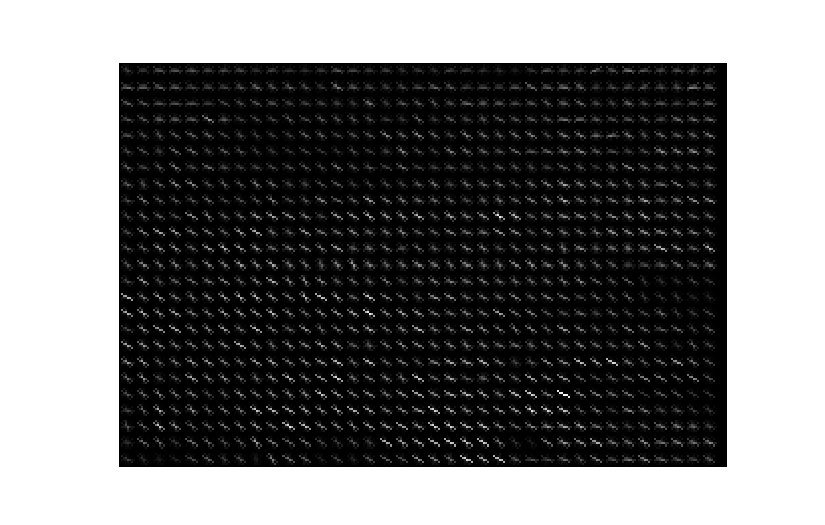
\includegraphics{results_files/figure-pdf/unnamed-chunk-15-5.pdf}

}

\end{figure}

\begin{Shaded}
\begin{Highlighting}[]
\NormalTok{plt.savefig(}\StringTok{\textquotesingle{}images/plots/grass2\_image\_hog.jpg\textquotesingle{}}\NormalTok{)}
\end{Highlighting}
\end{Shaded}

\begin{figure}[H]

{\centering 
\includegraphics{results_files/figure-pdf/unnamed-chunk-15-6.pdf}

}

\end{figure}

\hypertarget{polar-plot-of-angles-from-standard-hog}{%
\section{Polar Plot of Angles from Standard
HOG}\label{polar-plot-of-angles-from-standard-hog}}

\begin{Shaded}
\begin{Highlighting}[]
\NormalTok{grass2\_polar\_plot }\OtherTok{\textless{}{-}}
\FunctionTok{ggplot}\NormalTok{(hog\_df }\SpecialCharTok{\%\textgreater{}\%} \FunctionTok{filter}\NormalTok{(mag }\SpecialCharTok{\textgreater{}=} \FloatTok{0.1}\NormalTok{), }
       \FunctionTok{aes}\NormalTok{(}\AttributeTok{x =}\NormalTok{ radian)) }\SpecialCharTok{+}
  \FunctionTok{geom\_histogram}\NormalTok{(}\AttributeTok{colour =} \StringTok{"black"}\NormalTok{, }\AttributeTok{fill =} \StringTok{"lightblue"}\NormalTok{, }
                 \AttributeTok{breaks =} \FunctionTok{seq}\NormalTok{(}\DecValTok{0}\NormalTok{, }\DecValTok{2}\SpecialCharTok{*}\NormalTok{pi, }\AttributeTok{length.out =} \FloatTok{17.5}\NormalTok{),}
                 \AttributeTok{bins =} \DecValTok{9}\NormalTok{) }\SpecialCharTok{+}
  \FunctionTok{coord\_polar}\NormalTok{(}
    \AttributeTok{theta =} \StringTok{"x"}\NormalTok{, }\AttributeTok{start =} \DecValTok{0}\NormalTok{, }\AttributeTok{direction =} \DecValTok{1}\NormalTok{) }\SpecialCharTok{+}
  \FunctionTok{scale\_x\_continuous}\NormalTok{(}
    \AttributeTok{breaks =} \FunctionTok{c}\NormalTok{(}\DecValTok{0}\NormalTok{, pi}\SpecialCharTok{/}\DecValTok{4}\NormalTok{, pi}\SpecialCharTok{/}\DecValTok{2}\NormalTok{, }\DecValTok{3}\SpecialCharTok{*}\NormalTok{pi}\SpecialCharTok{/}\DecValTok{4}\NormalTok{, pi, }\DecValTok{5}\SpecialCharTok{*}\NormalTok{pi}\SpecialCharTok{/}\DecValTok{4}\NormalTok{, }\DecValTok{3}\SpecialCharTok{*}\NormalTok{pi}\SpecialCharTok{/}\DecValTok{2}\NormalTok{, }\DecValTok{7}\SpecialCharTok{*}\NormalTok{pi}\SpecialCharTok{/}\DecValTok{4}\NormalTok{), }
    \AttributeTok{labels =} \FunctionTok{c}\NormalTok{(}\StringTok{"N"}\NormalTok{, }\StringTok{"NE"}\NormalTok{, }\StringTok{"E"}\NormalTok{, }\StringTok{"SE"}\NormalTok{, }\StringTok{"S"}\NormalTok{, }\StringTok{"SW"}\NormalTok{, }\StringTok{"W"}\NormalTok{, }\StringTok{"NW"}\NormalTok{)}
\NormalTok{  )}\SpecialCharTok{+}
  \FunctionTok{labs}\NormalTok{(}\AttributeTok{title =} \StringTok{"Polar Plot of Internet Grass Image"}\NormalTok{) }\SpecialCharTok{+}
    \FunctionTok{theme\_minimal}\NormalTok{() }\SpecialCharTok{+}
  \FunctionTok{labs}\NormalTok{(}\AttributeTok{x =} \StringTok{""}\NormalTok{) }\SpecialCharTok{+}
  \FunctionTok{theme}\NormalTok{(}\AttributeTok{axis.title.y =} \FunctionTok{element\_blank}\NormalTok{(),}
        \AttributeTok{plot.title =} \FunctionTok{element\_text}\NormalTok{(}\AttributeTok{hjust =} \FloatTok{0.5}\NormalTok{))}

\NormalTok{grass2\_polar\_plot}
\end{Highlighting}
\end{Shaded}

\begin{figure}[H]

{\centering 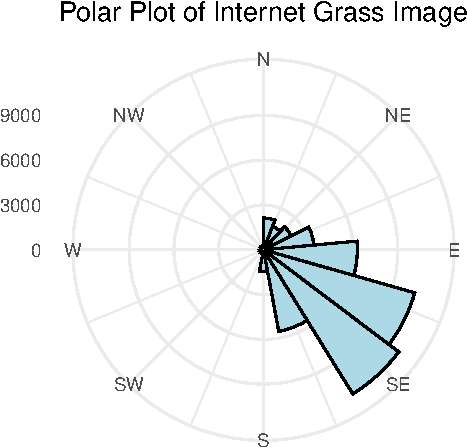
\includegraphics{results_files/figure-pdf/unnamed-chunk-16-9.pdf}

}

\end{figure}

\begin{Shaded}
\begin{Highlighting}[]
\CommentTok{\#ggsave("\_polar\_plot.jpg", polar\_plot, width = 6, height = 4, dpi = 300)}

\CommentTok{\#all\_plots \textless{}{-} ggpubr::ggarrange(diaganol\_polar\_plot, sf\_polar\_plot, grass2\_polar\_plot, aerial\_ll\_polar\_plot)}

\CommentTok{\#ggsave("images/plots/results\_all\_plots.jpg", all\_plots, width = 7, height = 7)}
\end{Highlighting}
\end{Shaded}

\hypertarget{hog-image-of-internet-grass}{%
\section{HOG Image of Internet
Grass}\label{hog-image-of-internet-grass}}

\begin{Shaded}
\begin{Highlighting}[]
\ImportTok{from}\NormalTok{ skimage }\ImportTok{import}\NormalTok{ color, io, exposure}
\ImportTok{from}\NormalTok{ skimage.transform }\ImportTok{import}\NormalTok{ resize}
\ImportTok{import}\NormalTok{ matplotlib.pyplot }\ImportTok{as}\NormalTok{ plt}
\ImportTok{from}\NormalTok{ skimage.feature }\ImportTok{import}\NormalTok{ hog}

\CommentTok{\# Load the image and preprocess it}
\NormalTok{img }\OperatorTok{=}\NormalTok{ color.rgb2gray(io.imread(}\StringTok{"images/grass\_image2.jpg"}\NormalTok{))}
\CommentTok{\# img = color.rgb2gray(io.imread("diagnol\_lines\_flipped.jpg"))}

\NormalTok{aspect\_ratio }\OperatorTok{=}\NormalTok{ img.shape[}\DecValTok{0}\NormalTok{] }\OperatorTok{/}\NormalTok{ img.shape[}\DecValTok{1}\NormalTok{]}
\NormalTok{height }\OperatorTok{=} \DecValTok{200}
\NormalTok{width }\OperatorTok{=} \BuiltInTok{int}\NormalTok{(height }\OperatorTok{/}\NormalTok{ aspect\_ratio)}
\NormalTok{resized\_img }\OperatorTok{=}\NormalTok{ resize(img, (height, width))}

\NormalTok{plt.figure(figsize}\OperatorTok{=}\NormalTok{(}\DecValTok{8}\NormalTok{, }\DecValTok{20}\NormalTok{))  }\CommentTok{\# Adjusted the figure size to accommodate the additional object}
\NormalTok{plt.imshow(resized\_img, cmap}\OperatorTok{=}\StringTok{"gray"}\NormalTok{)}
\NormalTok{plt.axis(}\StringTok{"off"}\NormalTok{)}
\end{Highlighting}
\end{Shaded}

\begin{verbatim}
(-0.5, 300.5, 199.5, -0.5)
\end{verbatim}

\begin{Shaded}
\begin{Highlighting}[]
\NormalTok{plt.show()}
\end{Highlighting}
\end{Shaded}

\begin{figure}[H]

{\centering 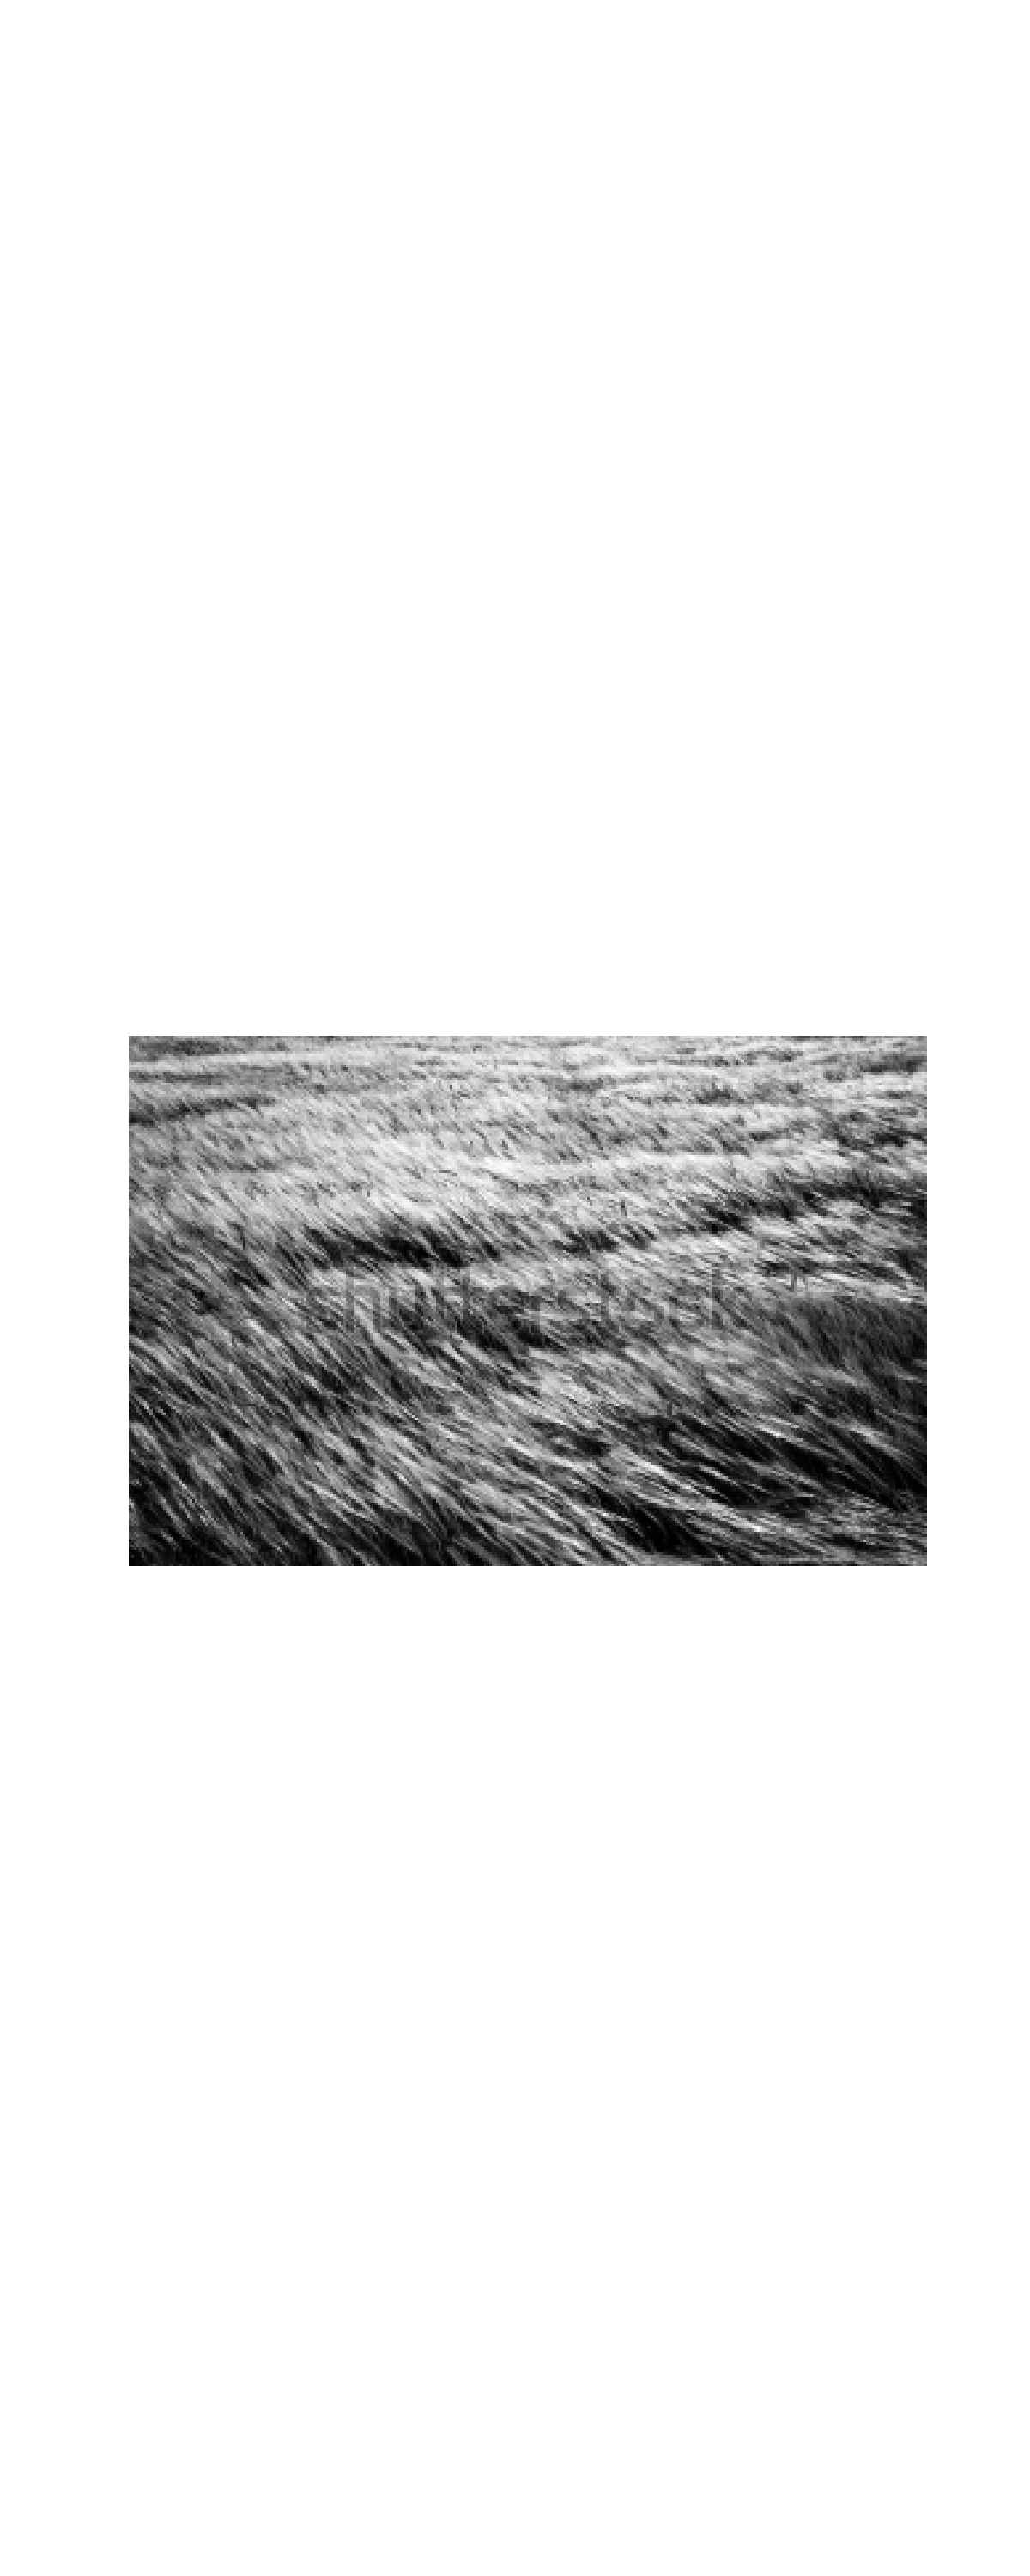
\includegraphics{results_files/figure-pdf/unnamed-chunk-17-1.pdf}

}

\end{figure}

\begin{Shaded}
\begin{Highlighting}[]
\CommentTok{\# Compute HOG features}
\NormalTok{hog\_features, hog\_image }\OperatorTok{=}\NormalTok{ hog(resized\_img, orientations}\OperatorTok{=}\DecValTok{9}\NormalTok{, pixels\_per\_cell}\OperatorTok{=}\NormalTok{(}\DecValTok{8}\NormalTok{,}\DecValTok{8}\NormalTok{),}
\NormalTok{                              cells\_per\_block}\OperatorTok{=}\NormalTok{(}\DecValTok{10}\NormalTok{, }\DecValTok{10}\NormalTok{), visualize}\OperatorTok{=}\VariableTok{True}\NormalTok{)}

\CommentTok{\# Plot the images}
\NormalTok{fig, (ax1, ax2, ax3) }\OperatorTok{=}\NormalTok{ plt.subplots(}\DecValTok{3}\NormalTok{, }\DecValTok{1}\NormalTok{, figsize}\OperatorTok{=}\NormalTok{(}\DecValTok{8}\NormalTok{, }\DecValTok{20}\NormalTok{), sharex}\OperatorTok{=}\VariableTok{True}\NormalTok{, sharey}\OperatorTok{=}\VariableTok{True}\NormalTok{)  }\CommentTok{\# Changed 1, 2 to 3, 1}

\CommentTok{\# Plot the rescaled black and white image}
\NormalTok{ax1.imshow(resized\_img, cmap}\OperatorTok{=}\NormalTok{plt.cm.gray)}
\NormalTok{ax1.set\_title(}\StringTok{\textquotesingle{}Rescaled Black and White Image\textquotesingle{}}\NormalTok{)}

\CommentTok{\# Plot the mag object}
\NormalTok{ax2.imshow(mag, cmap}\OperatorTok{=}\NormalTok{plt.cm.gray)  }\CommentTok{\# Assuming mag is the object you want to insert}
\CommentTok{\#ax2.axis("off")}
\NormalTok{ax2.set\_title(}\StringTok{\textquotesingle{}Pixel Magnitudes\textquotesingle{}}\NormalTok{)}

\CommentTok{\# rescale HOG for better viewing:}
\NormalTok{hog\_color\_rescaled }\OperatorTok{=}\NormalTok{ exposure.rescale\_intensity(hog\_image, in\_range}\OperatorTok{=}\NormalTok{(}\DecValTok{0}\NormalTok{, }\DecValTok{10}\NormalTok{))}

\CommentTok{\# Plot the histogram of oriented gradients}
\NormalTok{ax3.imshow(hog\_color\_rescaled, cmap}\OperatorTok{=}\NormalTok{plt.cm.gray)}
\NormalTok{ax3.set\_title(}\StringTok{\textquotesingle{}Histogram of Oriented Gradients (HOG)\textquotesingle{}}\NormalTok{)}

\NormalTok{plt.savefig(}\StringTok{"images/plots/rescaled\_grass2\_image\_hog.png"}\NormalTok{, dpi}\OperatorTok{=}\DecValTok{300}\NormalTok{)}

\NormalTok{plt.show()}
\end{Highlighting}
\end{Shaded}

\begin{figure}[H]

{\centering 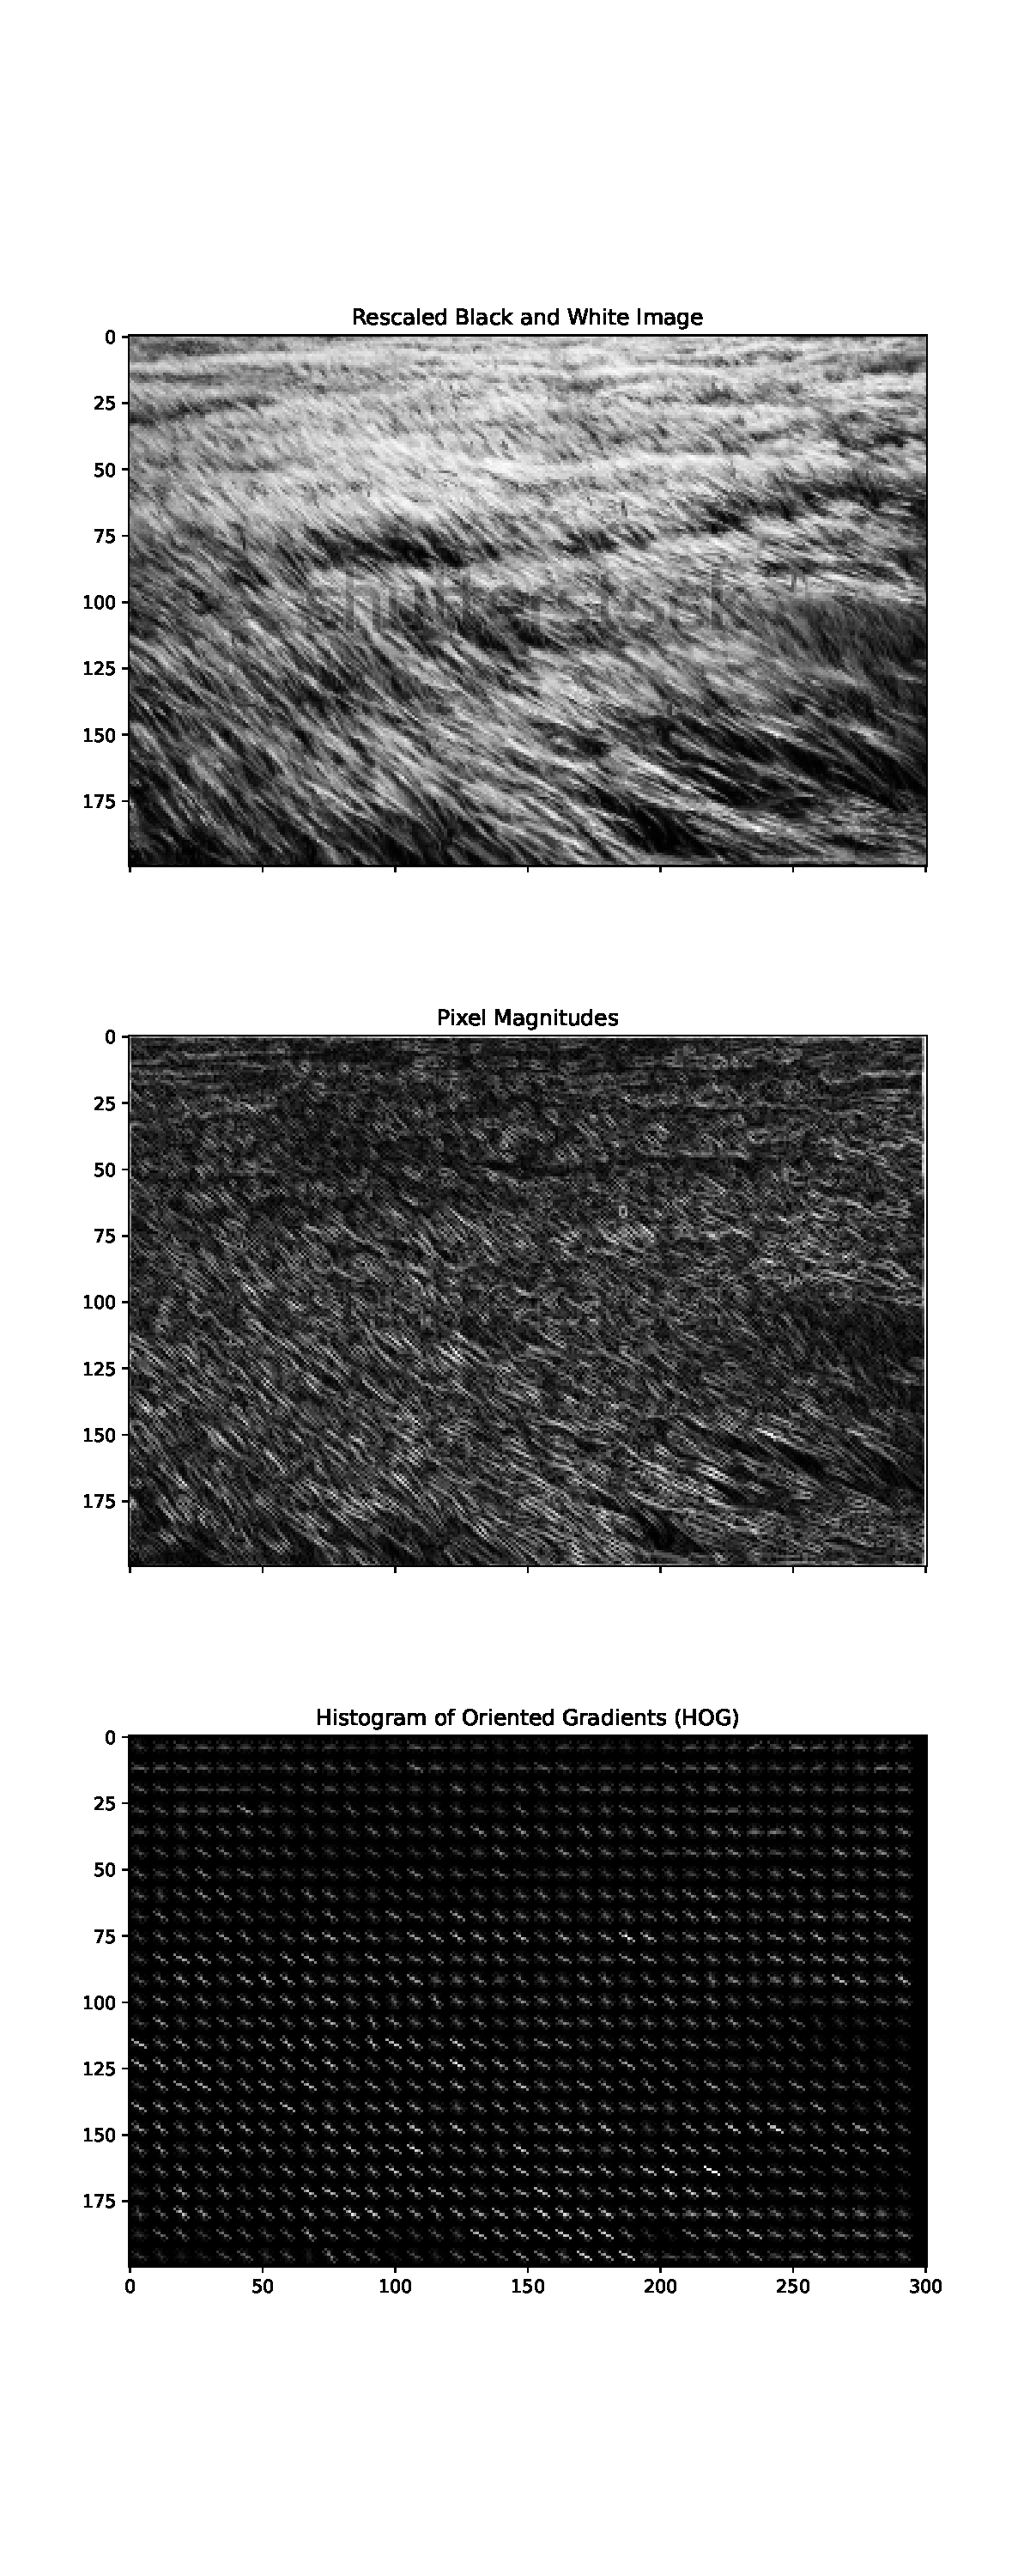
\includegraphics{results_files/figure-pdf/unnamed-chunk-17-2.pdf}

}

\end{figure}

\begin{Shaded}
\begin{Highlighting}[]
\ImportTok{from}\NormalTok{ skimage }\ImportTok{import}\NormalTok{ color, io, exposure}
\ImportTok{from}\NormalTok{ skimage.transform }\ImportTok{import}\NormalTok{ resize}
\ImportTok{import}\NormalTok{ matplotlib.pyplot }\ImportTok{as}\NormalTok{ plt}
\ImportTok{from}\NormalTok{ skimage.feature }\ImportTok{import}\NormalTok{ hog}

\CommentTok{\# Load the image and preprocess it}
\NormalTok{img }\OperatorTok{=}\NormalTok{ io.imread(}\StringTok{"images/grass\_image2.jpg"}\NormalTok{)}
\CommentTok{\# img = color.rgb2gray(io.imread("diagnol\_lines\_flipped.jpg"))}

\NormalTok{aspect\_ratio }\OperatorTok{=}\NormalTok{ img.shape[}\DecValTok{0}\NormalTok{] }\OperatorTok{/}\NormalTok{ img.shape[}\DecValTok{1}\NormalTok{]}
\NormalTok{height }\OperatorTok{=} \DecValTok{200}
\NormalTok{width }\OperatorTok{=} \BuiltInTok{int}\NormalTok{(height }\OperatorTok{/}\NormalTok{ aspect\_ratio)}
\NormalTok{resized\_img }\OperatorTok{=}\NormalTok{ resize(img, (height, width))}

\NormalTok{bw\_resized\_image }\OperatorTok{=}\NormalTok{ color.rgb2gray(resized\_img)}

\NormalTok{plt.figure(figsize}\OperatorTok{=}\NormalTok{(}\DecValTok{15}\NormalTok{, }\DecValTok{5}\NormalTok{))  }\CommentTok{\# Adjusted the figure size to accommodate the additional object}
\NormalTok{plt.imshow(resized\_img, cmap}\OperatorTok{=}\StringTok{"gray"}\NormalTok{)}
\NormalTok{plt.axis(}\StringTok{"off"}\NormalTok{)}
\end{Highlighting}
\end{Shaded}

\begin{verbatim}
(-0.5, 300.5, 199.5, -0.5)
\end{verbatim}

\begin{Shaded}
\begin{Highlighting}[]
\NormalTok{plt.show()}
\end{Highlighting}
\end{Shaded}

\begin{figure}[H]

{\centering 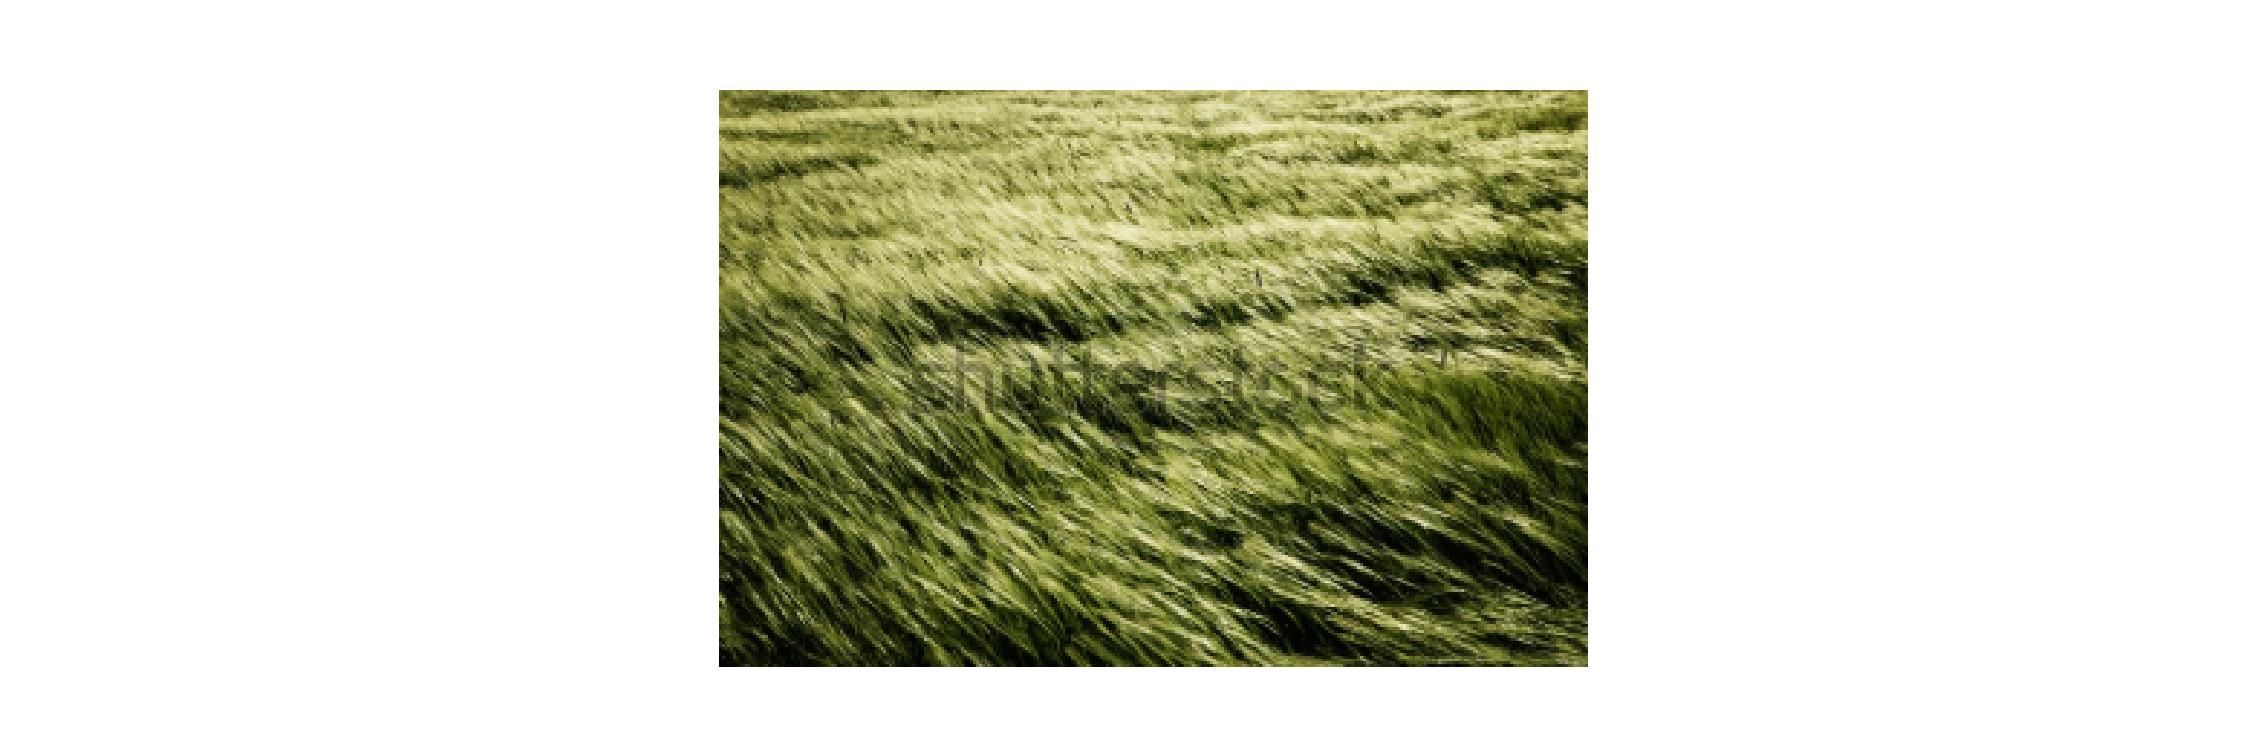
\includegraphics{results_files/figure-pdf/unnamed-chunk-18-5.pdf}

}

\end{figure}

\begin{Shaded}
\begin{Highlighting}[]
\CommentTok{\# Compute HOG features}
\NormalTok{hog\_features, hog\_image }\OperatorTok{=}\NormalTok{ hog(bw\_resized\_image, orientations}\OperatorTok{=}\DecValTok{9}\NormalTok{, pixels\_per\_cell}\OperatorTok{=}\NormalTok{(}\DecValTok{8}\NormalTok{,}\DecValTok{8}\NormalTok{),}
\NormalTok{                              cells\_per\_block}\OperatorTok{=}\NormalTok{(}\DecValTok{10}\NormalTok{, }\DecValTok{10}\NormalTok{), visualize}\OperatorTok{=}\VariableTok{True}\NormalTok{)}

\CommentTok{\# Plot the images}
\NormalTok{fig, (ax1, ax2, ax3) }\OperatorTok{=}\NormalTok{ plt.subplots(}\DecValTok{1}\NormalTok{, }\DecValTok{3}\NormalTok{, figsize}\OperatorTok{=}\NormalTok{(}\DecValTok{25}\NormalTok{, }\DecValTok{5}\NormalTok{), sharex}\OperatorTok{=}\VariableTok{True}\NormalTok{, sharey}\OperatorTok{=}\VariableTok{True}\NormalTok{)  }\CommentTok{\# Changed 3, 1 to 1, 5}

\CommentTok{\# Plot the rescaled input image}
\NormalTok{ax1.imshow(resized\_img, cmap}\OperatorTok{=}\NormalTok{plt.cm.gray)}
\NormalTok{ax1.set\_title(}\StringTok{\textquotesingle{}Rescaled Input Image\textquotesingle{}}\NormalTok{)}

\CommentTok{\# Plot the pixel magnitudes}
\NormalTok{ax2.imshow(mag, cmap}\OperatorTok{=}\NormalTok{plt.cm.gray)  }\CommentTok{\# Assuming mag is the object you want to insert}
\NormalTok{ax2.set\_title(}\StringTok{\textquotesingle{}Pixel Magnitudes\textquotesingle{}}\NormalTok{)}

\CommentTok{\# Plot the histogram of oriented gradients}
\NormalTok{hog\_color\_rescaled }\OperatorTok{=}\NormalTok{ exposure.rescale\_intensity(hog\_image, in\_range}\OperatorTok{=}\NormalTok{(}\DecValTok{0}\NormalTok{, }\DecValTok{10}\NormalTok{))}
\NormalTok{ax3.imshow(hog\_color\_rescaled, cmap}\OperatorTok{=}\NormalTok{plt.cm.gray)}
\NormalTok{ax3.set\_title(}\StringTok{\textquotesingle{}Histogram of Oriented Gradients (HOG) Image\textquotesingle{}}\NormalTok{)}

\CommentTok{\# Plot the histogram of oriented gradients}
\CommentTok{\# angle\_hist = io.imread("images/grass2\_angles\_histogram.jpg")}
\CommentTok{\# resized\_hist = resize(angle\_hist, (height, width))}
\CommentTok{\# ax4.imshow(resized\_hist, cmap=plt.cm.gray)}
\CommentTok{\# ax4.set\_title(\textquotesingle{}Angle Histogram\textquotesingle{})}
\CommentTok{\# }
\CommentTok{\# \# Plot the polar plot}
\CommentTok{\# polar\_plot = io.imread("images/grass2\_polar\_plot.jpg")}
\CommentTok{\# resized\_polar = resize(polar\_plot, (height, width))}
\CommentTok{\# ax5.imshow(resized\_polar, cmap=plt.cm.gray)}
\CommentTok{\# ax5.set\_title(\textquotesingle{}Polar Plot\textquotesingle{})}

\NormalTok{plt.savefig(}\StringTok{"images/plots/rescaled\_grass2\_image\_hog.png"}\NormalTok{, dpi}\OperatorTok{=}\DecValTok{300}\NormalTok{)}

\NormalTok{plt.show()}
\end{Highlighting}
\end{Shaded}

\begin{figure}[H]

{\centering 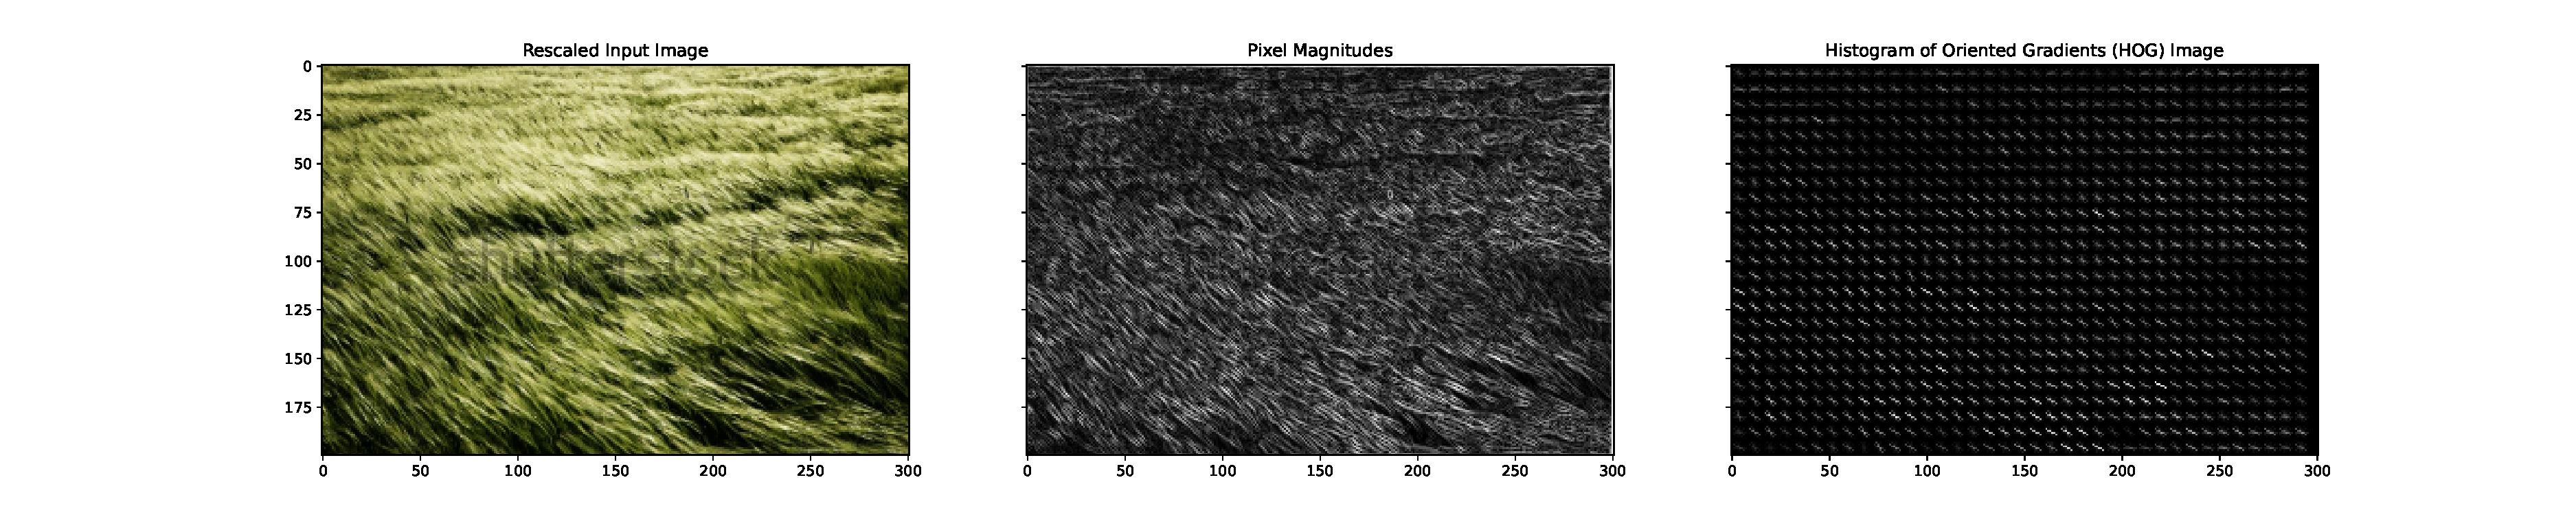
\includegraphics{results_files/figure-pdf/unnamed-chunk-18-6.pdf}

}

\end{figure}

\hypertarget{titus-flip}{%
\section{Titus Flip}\label{titus-flip}}

\begin{Shaded}
\begin{Highlighting}[]
\NormalTok{image }\OperatorTok{=}\NormalTok{ imread(}\StringTok{\textquotesingle{}images/TitusFlip.jpg\textquotesingle{}}\NormalTok{)}
\NormalTok{imshow(image)}
\BuiltInTok{print}\NormalTok{(image.shape)}
\end{Highlighting}
\end{Shaded}

\begin{verbatim}
(1350, 1080, 3)
\end{verbatim}

\begin{Shaded}
\begin{Highlighting}[]
\NormalTok{resized\_image }\OperatorTok{=}\NormalTok{ resize(image, (}\DecValTok{300}\NormalTok{, }\DecValTok{400}\NormalTok{))}
\CommentTok{\#resized\_image = image}
\NormalTok{imshow(resized\_image)}
\BuiltInTok{print}\NormalTok{(resized\_image.shape)}
\end{Highlighting}
\end{Shaded}

\begin{verbatim}
(300, 400, 3)
\end{verbatim}

\begin{Shaded}
\begin{Highlighting}[]
\NormalTok{fig, hog\_image }\OperatorTok{=}\NormalTok{ hog(resized\_image, orientations}\OperatorTok{=}\DecValTok{9}\NormalTok{, pixels\_per\_cell}\OperatorTok{=}\NormalTok{(}\DecValTok{3}\NormalTok{, }\DecValTok{3}\NormalTok{),}
\NormalTok{                     cells\_per\_block}\OperatorTok{=}\NormalTok{(}\DecValTok{15}\NormalTok{, }\DecValTok{15}\NormalTok{), visualize}\OperatorTok{=}\VariableTok{True}\NormalTok{, channel\_axis}\OperatorTok{=}\DecValTok{2} \CommentTok{\#multichannel=True}
\NormalTok{                     )}
\NormalTok{fig, (ax1, ax2) }\OperatorTok{=}\NormalTok{ plt.subplots(}\DecValTok{1}\NormalTok{, }\DecValTok{2}\NormalTok{, figsize}\OperatorTok{=}\NormalTok{(}\DecValTok{16}\NormalTok{, }\DecValTok{7}\NormalTok{), sharex}\OperatorTok{=}\VariableTok{True}\NormalTok{, sharey}\OperatorTok{=}\VariableTok{True}\NormalTok{)}

\NormalTok{ax1.imshow(resized\_image, cmap}\OperatorTok{=}\NormalTok{plt.cm.gray)}
\NormalTok{ax1.set\_title(}\StringTok{\textquotesingle{}Input image\textquotesingle{}}\NormalTok{)}

\CommentTok{\# Rescale histogram for better display }
\NormalTok{hog\_color\_rescaled }\OperatorTok{=}\NormalTok{ exposure.rescale\_intensity(hog\_image, in\_range}\OperatorTok{=}\NormalTok{(}\DecValTok{0}\NormalTok{, }\DecValTok{10}\NormalTok{))}

\NormalTok{ax2.imshow(hog\_color\_rescaled, cmap}\OperatorTok{=}\NormalTok{plt.cm.gray)}
\NormalTok{ax2.set\_title(}\StringTok{\textquotesingle{}Histogram of Oriented Gradients (HOG)\textquotesingle{}}\NormalTok{)}

\CommentTok{\# store to file}
\NormalTok{plt.savefig(}\StringTok{"images/plots/titus\_flip\_example\_hog.png"}\NormalTok{, dpi}\OperatorTok{=}\DecValTok{300}\NormalTok{)}

\NormalTok{plt.show()}
\end{Highlighting}
\end{Shaded}

\begin{figure}[H]

{\centering 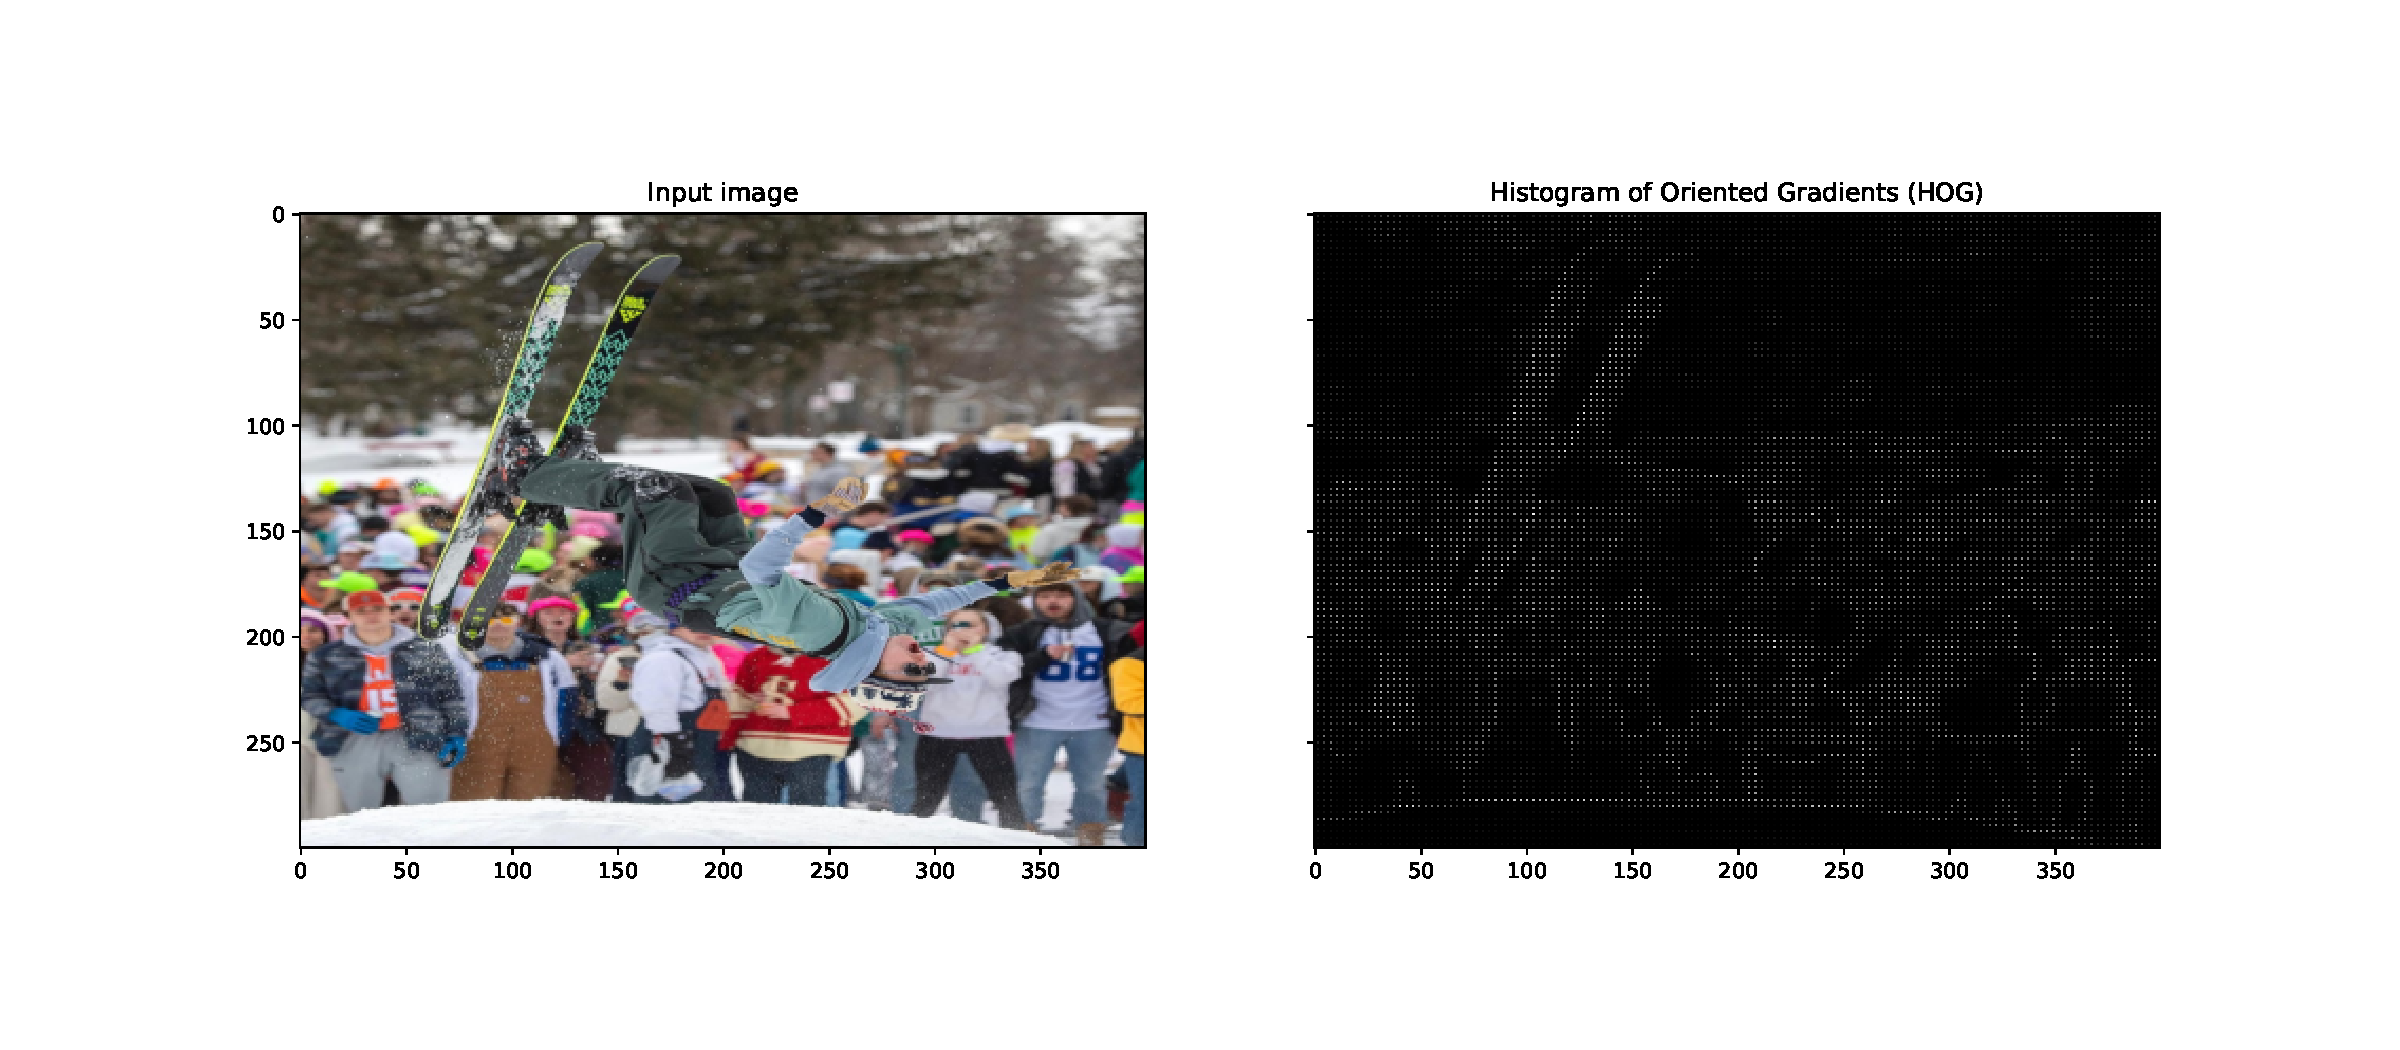
\includegraphics{results_files/figure-pdf/unnamed-chunk-19-9.pdf}

}

\end{figure}

\begin{figure}[H]

{\centering 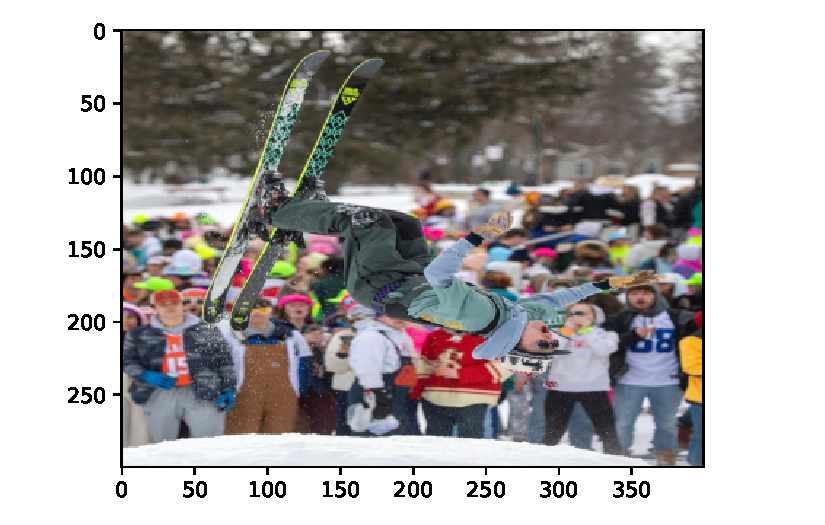
\includegraphics{results_files/figure-pdf/unnamed-chunk-19-10.pdf}

}

\end{figure}

\begin{Shaded}
\begin{Highlighting}[]
\CommentTok{\# hog\_df \textless{}{-} py$hog\_df}


\CommentTok{\# ggplot(hog\_df \%\textgreater{}\% filter(mag \textgreater{}= 0.4), }
\CommentTok{\#        aes(x = radian)) +}
\CommentTok{\#   geom\_histogram(\#binwidth = 5\#, boundary = 0, closed = "right") +}
\CommentTok{\#   )+}
\CommentTok{\#   \#scale\_x\_continuous(limits = c(0, 360), breaks = seq(0, 360, by = 45)) +}
\CommentTok{\#   \#coord\_polar(start = 0, direction = 1, ) +}
\CommentTok{\#   coord\_radial(start = 0, end = pi, expand = F, clip = "on") +}
\CommentTok{\#   scale\_x\_continuous(}
\CommentTok{\#     breaks = c(0, pi/4, pi/2, 3*pi/4), }
\CommentTok{\#     labels = c("0", "π/4", "π/2", "3π/4")}
\CommentTok{\#   ) +}
\CommentTok{\#   theme(plot.title = element\_text(hjust = 0.5)) +}
\CommentTok{\#   labs(title = "Polar Histogram of Theta",}
\CommentTok{\#        x = "Theta (Degrees)",}
\CommentTok{\#        y = "Frequency") \#+ theme\_minimal()}
\end{Highlighting}
\end{Shaded}

\bookmarksetup{startatroot}

\hypertarget{conclusion}{%
\chapter{Conclusion}\label{conclusion}}



\end{document}
